\باب{ٹرانسفارمر}
ٹرانسفارمر وہ آلہ ہے جو بدلتی برقی دباو تبدیل کرتا ہے۔ یہ دو یا دو سے زیادہ لچھوں پر مشتمل ہوتا ہے جو مقناطیسی قالب\فرہنگ{مقناطیسی قالب}\حاشیہب{magnetic core}\فرہنگ{core} پر لپٹے ہوتے ہیں۔یہ لچھے عموماً آپس میں جُڑے ہوئے نہیں ہوتے۔شکل \حوالہ{شکل_ٹرانسفارمر_علامت}-الف میں ٹرانسفارمر کی علامت دکھائی گئی ہے۔دو لچھوں کے درمیان متوازی لکیریں مقناطیسی قالب کو ظاہر کرتی ہیں۔

دستیاب برقی دباو\حاشیہد{بدلتی برقی دباو کی علامت میں مثبت اور منفی نشان وقت صفر پر برقی دباو کی مثبت اور منفی سرے ظاہر کرتے ہیں۔} پر ٹرانسفارمر کے ایک لچھے کو برقی طاقت فراہم کی جاتی ہے اور باقی لچھوں سے  مختلف برقی دباو پر یہی برقی طاقت حاصل کی جاتی ہے۔جس لچھے پر برقی دباو لاگو کیا جائے اسے \اصطلاح{ابتدائی لچھا}\فرہنگ{لچھا!ابتدائی}\فرہنگ{ابتدائی!لچھا}\حاشیہب{primary coil}\فرہنگ{coil!primary}  کہتے ہیں اور ٹرانسفارمر کی اس جانب کو \اصطلاح{ابتدائی جانب}\فرہنگ{ابتدائی!جانب}\حاشیہب{primary side}\فرہنگ{primary!side} کہتے ہیں۔اسی طرح جس لچھے (لچھوں) سے برقی طاقت حاصل کی جاتی ہے اسے (انہیں) \اصطلاح{ثانوی لچھا}\فرہنگ{لچھا!ثانوی}\حاشیہب{secondary coil}\فرہنگ{coil!secondary}  (لچھے) کہتے ہیں اور اس جانب کو \اصطلاح{ثانوی جانب}\فرہنگ{ثانوی جانب}\فرہنگ{side!secondary}\حاشیہب{secondary side}  کہتے ہیں۔یہ شکل کے حصہ با میں دکھایا گیا ہے۔ٹرانسفارمر کی ابتدائی جانب کو بائیں ہاتھ کی جانب اور ثانوی جانب کو دائیں ہاتھ کی جانب بنایا جاتا ہے۔
\begin{figure}
\centering
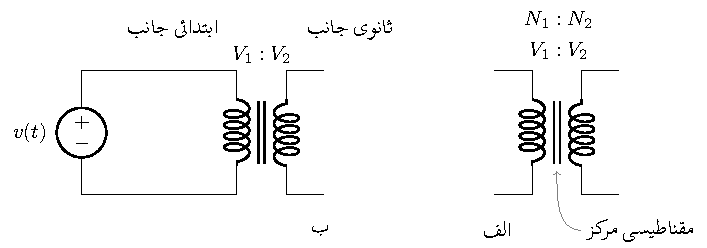
\includegraphics{figTransformersSymbol}
\caption{ٹرانسفارمر کی علامت۔}
\label{شکل_ٹرانسفارمر_علامت}
\end{figure}

بڑے ٹرانسفارمر عموماً دو ہی لچھوں پر مشتمل ہوتے ہیں۔اس کتاب میں ہم دو ہی لچھوں کے مقناطیسی قالب پر لپٹے قوی ٹرانسفارمر پر تبصرہ کریں گے۔

	ٹرانسفارمر کے کم برقی دباو کے لچھے کو \اصطلاح{کم برقی دباو کا لچھا}\فرہنگ{لچھا!کم برقی دباو}\حاشیہب{low voltage coil}\فرہنگ{coil!low voltage}  کہتے ہیں اور ٹرانسفارمر کی اس جانب کو \اصطلاح{کم برقی دباو والی جانب}  کہتے ہیں جبکہ اس کے زیادہ برقی دباو کے لچھے کو \اصطلاح{زیادہ برقی دباو کا لچھا}\فرہنگ{لچھا!زیادہ برقی دباو}\حاشیہب{high voltage coil}\فرہنگ{coil!high voltage}  کہتے ہیں اور ٹرانسفارمر کی اس جانب کو \اصطلاح{زیادہ برقی دباو والی جانب}  کہتے ہیں۔

یوں اگر ٹرانسفارمر کے کم برقی دباو کی جانب برقی دباو لاگو کیا جائے اور زیادہ برقی دباو کی جانب سے برقی دباو حاصل کیا جائے تو ٹرانسفارمر کی کم برقی دباو والی جانب کو ابتدائی جانب کہیں گے اور اس کی زیادہ برقی دباو والی جانب کو ثانوی جانب کہیں گے۔

\حصہ{ٹرانسفارمر کی اہمیت}
بدلتی رو کی برقی طاقت اتنی مقبول اس لئے ہوئی ہے کہ یہ ایک جگہ سے دوسری جگہ با آسانی اور نہایت کم برقی طاقت کی ضیاع کے ساتھ منتقل کی جا سکتی ہے۔ٹرانسفارمر کی تبادلہ برقی دباو\فرہنگ{برقی دباو!تبادلہ}\حاشیہب{voltage transformation property} کی خصوصیت ایسا کرنے میں کلیدی کردہر ادا کرتی ہے۔ یہ ایک مثال سے بہتر سمجھا جا سکتا ہے۔
%
\ابتدا{مثال}
شکل \حوالہ{شکل_ٹرانسفارمر_برقی_طاقت_منتقلی}  سے رجوع کریں۔برقی دباو اور برقی رو کی حاصلِ ضرب برقی طاقت ہوتی ہے یعنی
\begin{figure}
\centering
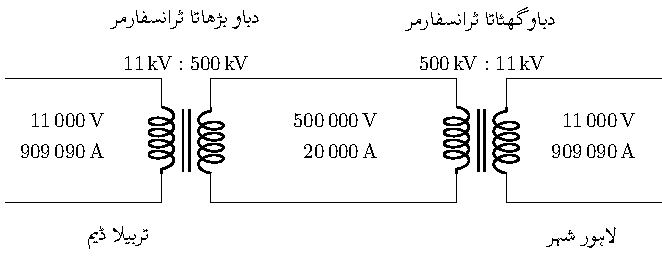
\includegraphics{figTransformersVoltageStepUpBenefits}
\caption{برقی طاقت کی منتقلی۔}
\label{شکل_ٹرانسفارمر_برقی_طاقت_منتقلی}
\end{figure}

%
\begin{align*}
p=v_1 i_1 = v_2 i_2
\end{align*}
اب تصور کریں کہ تربیلا ڈیم \عددیء{10,000,000,000} واٹ یعنی دس گیگا واٹ\حاشیہب{Giga Watt}  برقی طاقت پیدا کر رہا ہے اور اس طاقت کو لاہور\حاشیہد{ضلع صوابی میں بھی لاہور ایک تحصیل ہے لیکن اس شہر کو اتنی طاقت نہیں درکار } شہر منتقل کرنا ہے جہاں گھریلو صارفین کو یہ \عددیء{220} وولٹ پر مہیا کرنی ہے۔اگر ہم اس طاقت کو \عددیء{220}  وولٹ پر ہی منتقل کرنا چاہیں تو برقی رو
\begin{align*}
i=\frac{p}{v}=\frac{\num{10000000000}}{220}=\SI{45454545}{\ampere}
\end{align*}
ہو گی۔برقی تار میں کثافتِ برقی رو \عددیء{J_{au}} تقریباً \عددیء{5} ایمپیئر فی مربع ملی میٹر \عددیء{J_{au}=\SI{5}{\ampere \per \milli\meter \squared}}  ممکن ہوتی ہے۔یہ ایک محفوظ کثافتِ برقی رو ہے۔اگر برقی تار میں اس سے زیادہ برقی رو گزاری جائے تو اس کی مزاحمت میں برقی طاقت کے ضیاع سے یہ گرم ہو کر پگھل سکتی ہے۔ اس طرح صفحہ \حوالہصفحہ{مساوات_بنیادی_برقی_رو_کثافت} پر  مساوات \حوالہ{مساوات_بنیادی_برقی_رو_کثافت} سے برقی تار کا رقبہ عمودی تراش
\begin{align*}
A=\frac{i}{J_{au}}=\frac{45454545}{5}=\SI{9090909}{\milli\meter\squared}
\end{align*}
ہو گا۔ گول تار تصور کریں تو اس کا رداس
\begin{align*}
r=\sqrt{\frac{A}{\pi}}=\sqrt{\frac{9090909}{\pi}}=\SI{1701}{\milli\meter}=\SI{1.7}{\meter}
\end{align*}
حاصل ہوتی ہے۔آپ نے دیکھا کہ درکار برقی تار کا رداس \عددیء{1.7} میٹر ہے۔اتنی موٹی برقی تار کہیں نہیں پائی جاتی ہے\حاشیہد{آپ مانیں یا نہ مانیں، آپ نے بھی اتنی موٹی برقی تار کبھی نہیں دیکھی}۔اگر یہ تار المونیم کی بنی ہو جس کی  کثافت  \عددیء{\rho_v=\SI{2700}{\kilo\gram\per\meter\squared}} ہے تو ایک میٹر لمبی تار کی کمیت
\begin{align*}
m=2700 \times \pi \times 1.7^2 \times 1=\SI{24513}{\kilo\gram}
\end{align*}
یعنی \عددیء{24} ٹن ہو گی۔المونیم اتنی مہنگی ہے کہ اس صورت میں اتنی برقی طاقت کو لاہور پہنچانا ممکن نہیں\حاشیہد{آج کل لاہور میں لوڈ شیدنگ اس وجہ سے نہیں}۔

ڈیم پر ایک ٹرانسفارمر نسب کیا جائے جو برقی دباو کو بڑھا کر  \عددیء{\num{500000}} وولٹ یعنی \عددیء{500} کلو وولٹ  کر دے تب صرف 
\begin{align*}
i=\frac{p}{v}=\frac{\num{10000000000}}{\num{500000}}=\SI{20000}{\ampere}
\end{align*}
ایمپیئر درکار ہوں گے جس کے لئے درکار برقی تار
\begin{align*}
A&=\frac{i}{J_{au}}=\frac{\num{20000}}{5}=\SI{4000}{\milli\meter\squared}\\
r&=\sqrt{\frac{A}{\pi}}=\sqrt{\frac{4000}{\pi}}=\SI{35.7}{\milli\meter}
\end{align*}
صرف \عددیء{35} ملی میٹر رداس کی ہو گی۔
\انتہا{مثال}
%

اس مثال میں اگر تربیلا ڈیم میں نسب جنریٹر \عددیء{11000} وولٹ برقی دباو پیدا کر رہا ہو تو تربیلا ڈیم  پر نسب  ٹرانسفارمر برقی دباو کو \عددیء{11000} وولٹ سے بڑھا کر \عددیء{500} کلو وولٹ کرے گا جبکہ لاہور شہر میں نسب  ٹرانسفارمر اس برقی دباو کو \عددیء{500} کلو وولٹ سے واپس \عددیء{11000} وولٹ کر دے گا۔

اسی مثال کو مزید آگے لے جاتے ہیں۔شہر میں \عددیء{220} وولٹ کی بجائے \عددیء{11000} وولٹ صارف تک پہنچائے جائیں گے اور۔وہیں نزدیک ایک اور ٹرانسفارمر  \عددیء{11000}  وولٹ کو مزید گھٹا کر صارف کو  \عددیء{220} وولٹ فراہم کرے گی۔ 

شکل \حوالہ{شکل_ٹرانسفارمر_برقی_طاقت_منتقلی} میں ڈیم سے شہر تک کا نظام دکھایا گیا ہے جہاں ڈیم پر نسب ٹرانسفارمر کو \اصطلاح{برقی دباو بڑھاتا ٹرانسفارمر}\فرہنگ{ٹرانسفارمر!دباو بڑھاتا}\حاشیہب{step up transformer}\فرہنگ{step up transformer}  اور لاہور میں نسب ٹرانسفارمر کو \اصطلاح{برقی دباو گھٹاتا ٹرانسفارمر}\فرہنگ{ٹرانسفارمر!دباو گھٹاتا}\حاشیہب{step down transformer}\فرہنگ{step down transformer}  کہا گیا ہے۔

برقی طاقت عموماً \عددیء{11} کلو وولٹ اور  \عددیء{25} کلو وولٹ کے مابین پیدا کی جاتی ہے۔اس کی منتقلی  \عددیء{110 } کلو وولٹ اور \عددیء{1000}  کلو وولٹ کے مابین کی جاتی ہے جبکہ اس کا استعمال  \عددیء{1000} وولٹ سے کم پر کیا جاتا ہے۔

\حصہ{ٹرانسفارمر کے اقسام}
گھروں اور کارخانوں کو برقی طاقت فراہم کرنے والے ٹرانسفارمر مقناطیسی قالب پر لپٹے جاتے ہیں۔یہ عموماً  \اصطلاح{تین مرحلہ}\فرہنگ{تین مرحلہ}\حاشیہب{three phase}\فرہنگ{three phase} ہوتے ہیں۔ اور انہیں \اصطلاح{لوہے کے قالب والے تین  مرحلہ قوی ٹرانسفارمر}\حاشیہب{iron core, three phase power transformer} کہتے ہیں۔

نہایت چھوٹے ٹرانسفارمر عموماً لوہے کے قالب اور \اصطلاح{ایک مرحلہ}\فرہنگ{ایک مرحلہ}\حاشیہب{single phase}\فرہنگ{single phase} ہوتے ہیں۔یہ گھریلو استعمال کے برقی مشین، مثلاً موبائل چارجر، میں لگے ہوتے ہیں اور \عددیء{220} وولٹ سے برقی دباو مزید گھٹاتے ہیں۔

کچھ ٹرانسفارمر اس طرح بنائے جاتے ہیں کہ ان کی ثانوی جانب برقی دباو ان کی ابتدائی جانب برقی دباو کی خاص نسبت سے ہو۔یہ نسبت حاصل کرنے پر خاص توجہ دی جاتی ہے۔ انہیں  \اصطلاح{دباو کے ٹرانسفارمر}\فرہنگ{ٹرانسفارمر!برقی دباو، میٹر}\حاشیہب{potential transformer}  کہتے ہیں۔اسی طرح کچھ ٹرانسفارمر اس طرح بنائے جاتے ہیں کہ ان کی ثانوی جانب برقی رو، ابتدائی جانب برقی رو کی خاص نسبت سے ہو۔ یہ نسبت حاصل کرنے پر خاص توجہ دی جاتی ہے۔ان کو \اصطلاح{رو کے ٹرانسفارمر}\فرہنگ{ٹرانسفارمر!رو، میٹر}\حاشیہب{current transformer}  کہتے ہیں۔یہ دو قسم کے ٹرانسفارمر برقی دباو اور برقی رو ناپنے کے لئے استعمال ہوتے ہیں۔ ویسے تو ہر ٹرانسفارمر کسی نسبت سے ہی برقی دباو یا برقی رو کم یا زیادہ کرتا ہے لیکن جیسا پہلے ذکر ہوا ان دو قسم کے ٹرانسفارمروں میں کم اور زیادہ کرنے کی نسبت پر خاص توجہ رکھی جاتی ہے۔ان دو اقسام کے ٹرانسفارمروں کی برقی سکت\فرہنگ{برقی سکت}\حاشیہب{electrical rating}\فرہنگ{electrical rating} نہایت کم\حاشیہد{یہ عموماً تقریباً پچیس وولٹ-ایمپیئر سکت رکھتے ہیں۔} ہوتی ہے۔

ٹرانسفارمر کے لچھوں کے مابین مشترکہ مقناطیسی بہاو خلاء کے ذریعہ بھی ممکن ہے۔انہیں \اصطلاح{خلائی قالب ٹرانسفارمر}\فرہنگ{ٹرانسفارمر!خلائی قالب}\حاشیہب{air core transformer}\فرہنگ{transformer!air core}  کہتے ہیں۔ ایسے ٹرانسفارمر ذرائع ابلاغ\فرہنگ{ٹرانسفارمر!ذرائع ابلاغ}\حاشیہب{communication transformer}\فرہنگ{transformer!communication} کے ادوار، یعنی ریڈیو، ٹی وی وغیرہ میں پائے جاتے ہیں۔ان ٹرانسفارمروں کی علامت  شکل  الف کی طرح ہوتی ہے مگر اس میں مقناطیسی قالب ظاہر کرنے والی متوازی لکیریں نہیں ہوتیں۔

\حصہ{امالی برقی دباو}\شناخت{حصہ_ٹرانسفارمر_امالی_برقی_دباو}
اس حصے کا بنیادی مقصد بیرونی برقی دباو \عددیء{v}  اور اندرونی امالی برقی دباو  \عددیء{e} میں فرق واضح کرنا اور اس سے تعلق رکھنے والی تکنیکی اصطلاح کا تعارف کرانا ہے۔

شکل  \حوالہ{شکل_ٹرانسفارمر_بیرونی_اور_اندرونی_برقی_دباو} میں بے بوجھ\فرہنگ{بے بوجھ}\حاشیہب{unloaded} ٹرانسفارمر دکھایا گیا ہے یعنی اس کے ثانوی لچھے کو کھلے دور رکھا گیا ہے۔ابتدائی لچھے پر \عددیء{v_1} برقی دباو لاگو کرنے سے ابتدائی لچھے میں ہیجان انگیز\فرہنگ{ہیجان انگیز برقی رو}\حاشیہب{excitation current}\فرہنگ{excitation current} برقی رو \عددیء{i_{\varphi}} گزرے گی۔اس ہیجان انگیز برقی رو سے پیدا مقناطیسی دباو \عددیء{N_1 i_{\varphi}}  قالب میں مقناطیسی بہاو  \عددیء{\varphi} کو جنم دے گی۔ یہ بدلتی مقناطیسی بہاو ابتدائی لچھے میں امالی برقی  دباو \عددیء{e_1}  پیدا کرتی ہے جہاں
\begin{align}
e_1=-\frac{\dif \lambda}{\dif t}=-N_1 \frac{\dif \varphi}{\dif t}
\end{align}

 اس مساوات میں
\begin{itemize}
\item
\عددیء{\lambda} ابتدائی لچھے کی مقناطیسی بہاو کے ساتھ ارتباط بہاو ہے
\item
\عددیء{\varphi} مقناطیسی قالب میں مقناطیسی بہاو جو دونوں لچھوں میں سے گزرتی ہے
\item
\عددیء{N_1} ابتدائی لچھے کے چکر
\end{itemize}
%
\begin{figure}
\centering
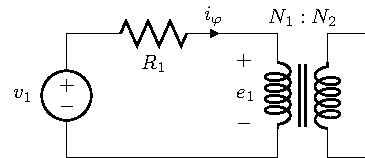
\includegraphics{figTransformersAppliedAndInducedVoltages}
\caption{بیرونی برقی دباو اور اندرونی امالی برقی دباو میں فرق۔}
\label{شکل_ٹرانسفارمر_بیرونی_اور_اندرونی_برقی_دباو}
\end{figure}

اگر اس ابتدائی لچھے کی برقی تار کی مزاحمت \عددیء{R_1} ہو تب کرخوف کے قانون برائے برقی دباو سے
\begin{align}\label{مساوات_ٹرانسفارمر_بیرونی_اندرونی_دباو_فرق}
v_1 = i_{\varphi} R_1+e_1
\end{align}

شکل میں اس مزاحمت کو ٹرانسفارمر کے باہر دکھایا گیا ہے۔اس لچھے کی رِستا متعاملہ بھی ہوتی ہے لیکن اسے یہاں نظرانداز کیا گیا ہے۔عام تر طاقت کے ٹرانسفارمر اور موٹروں  میں \عددیء{i_{\varphi} R_1} کی قیمت \عددیء{e_1} اور \عددیء{v_1} سے بہت کم ہوتی ہے لہٰذا اسے نظرانداز کیا جا سکتا ہے۔ ایسا کرنے سے ہم لکھ سکتے ہیں 
\begin{align}\label{مساوات_ٹرانسفارمر_بیرونی_اندرونی_دباو_تقریبا_برابر}
v_1 = e_1=-N_1 \frac{\dif \varphi}{\dif t}
\end{align}

مساوات \حوالہ{مساوات_ٹرانسفارمر_بیرونی_اندرونی_دباو_فرق} سے یہ ثابت ہوتا ہے کہ بیرونی لاگو برقی دباو \عددیء{v_1} اور اندرونی امالی برقی دباو \عددیء{e_1} دو علیحدہ برقی دباو ہیں۔یہ بات سمجھ لینا بہت ضروری ہے۔مساوات \حوالہ{مساوات_ٹرانسفارمر_بیرونی_اندرونی_دباو_تقریبا_برابر} کے تحت ان دو برقی دباو کی غیر سمتیں عموماً برابر ہوتی ہیں۔\حاشیہد{جس سے طلباء کو یہ غلط فہمی لاحق ہو جاتی ہے کہ یہ ایک ہی برقی دباو کے دو نام ہیں۔}اس کتاب میں عموماً مساوات \حوالہ{مساوات_ٹرانسفارمر_بیرونی_اندرونی_دباو_تقریبا_برابر}  کی طرح مساواتوں میں دائیں جانب منفی کی علامت نہیں لکھی گئی ۔عموماً برقی دباو کی قیمت درکار ہوتی ہے نا کہ اس کی علامت۔

لچھا \اصطلاح{ہیجان}\فرہنگ{ہیجان}\حاشیہب{excitation}\فرہنگ{excitation} کرنے سے مراد اس پر بیرونی برقی دباو لاگو کرنا  جبکہ لچھے پر لاگو بیرونی برقی دباو کو \اصطلاح{ہیجان انگیز برقی دباو}\فرہنگ{ہیجان انگیز!برقی دباو}\حاشیہب{excitation voltage}\فرہنگ{excitation voltage}  کہتے ہیں۔لچھے  کو \اصطلاح{ہیجان شدہ} لچھا\فرہنگ{ہیجان!لچھا}\حاشیہب{excited coil}\فرہنگ{excited coil} جبکہ اس میں رواں برقی رو کو \اصطلاح{ہیجان انگیز برقی رو}\فرہنگ{ہیجان انگیز!برقی رو}\فرہنگ{excitation current}\حاشیہب{excitation current} کہتے ہیں۔

برقی دباو عموماً لچھے سے گزرتی مقناطیسی بہاو کی تبدیلی سے حاصل کی جاتی ہے۔اگر ایسا کرتے لچھا ساکن رہے، جیسا کہ ٹرانسفارمر میں ہوتا ہے، تب حاصل برقی دباو کو \اصطلاح{امالی برقی دباو}\فرہنگ{امالی برقی دباو}\حاشیہب{induced voltage}\فرہنگ{induced voltage}  کہتے ہیں۔اگر برقی دباو کا حصول مقناطیسی میدان میں لچھے کی حرکت سے ممکن بنایا جائے تب اسے  \اصطلاح{محرک برقی دباو}\فرہنگ{محرک برقی دباو}\حاشیہب{electromotive force, emf}\فرہنگ{electromotive force}  کہتے ہیں۔یاد رہے ان برقی دباو میں کسی قسم کا فرق نہیں ہوتا۔انہیں مختلف نام صرف پہچان کی خاطر دئے جاتے ہیں۔

\حصہ{ہیجان انگیز  برقی رو اور قالبی ضیاع}
جہاں مقناطیسی قالب میں بدلتی مقناطیسی بہاو ثانوی لچھوں میں فائدہ مند برقی دباو پیدا کرتی ہے وہاں یہ مقناطیسی قالب میں نقصان دہ برقی دباو کو بھی جنم دیتی ہے جس سے مقناطیسی قالب میں \اصطلاح{بھنور نما برقی رو}\فرہنگ{بھنور نما!برقی رو}\حاشیہب{eddy currents}\فرہنگ{eddy currents} پیدا ہوتی ہے۔ اس بھنور نما برقی رو کی وجہ سے مقناطیسی قالب میں برقی طاقت کا ضیاع ہوتا ہے جسے \اصطلاح{بھنور نما برقی رو کا ضیاع}\فرہنگ{بھنور نما!ضیاع}\حاشیہب{eddy current loss}\فرہنگ{eddy current loss}  یا \اصطلاح{قالبی ضیاع}\فرہنگ{قالبی ضیاع}\حاشیہب{core loss}\فرہنگ{core loss} کہتے ہیں۔ اس برقی طاقت  کے ضیاع کو کم سے کم کرنے کیلئے مقناطیسی قالب کو  باریک لوہے کی \اصطلاح{پتریاں}\فرہنگ{پتریاں}\حاشیہب{laminations}\فرہنگ{laminations} تہہ در تہہ رکھ کر بنایا جاتا ہے۔ان پتریوں پر غیر موصل روغن\فرہنگ{روغن}\حاشیہب{enamel}\فرہنگ{enamel} کی تہہ لگائی جاتی ہے تا کہ بھنور نما برقی رو کو روکا جا سکے۔آپ دیکھیں گے کہ برقی مشین کا قالب عموماً اسی طرح بنایا جاتا ہے۔شکل \حوالہ{شکل_مقناطیسی_ادوار_ایم_پانچ_پتری_کا_خط} اور جدول \حوالہ{جدول_مقناطیسی_ادوار_کثافت_بہاو_بالمقابل_شدت}  میں \عددیء{0.3048} ملی میٹر موٹی \تحریر{M5} قالبی پتری کی \عددیء{B-H} مواد دی گئی ہے۔

قالبی پتریاں عموماً دو اشکال کی ہوتی ہیں۔یہ شکل \حوالہ{شکل_ٹرانسفارم_تہہ_در_تہہ_مرکز}-الف میں دکھایا گیا ہے۔ان کی شکل کی وجہ سے یہ \اصطلاح{ایک} شکل اور \اصطلاح{تین}\فرہنگ{ایک، تین پتریاں}\حاشیہب{E,I}\فرہنگ{E,I} شکل کی پتریاں کہلاتے ہیں۔ شکل \حوالہ{شکل_ٹرانسفارم_تہہ_در_تہہ_مرکز}-ب میں ایک اور تین  کو دو طرح آپس میں رکھا گیا ہے۔ان دو طریقوں سے انہیں تہہ در تہہ رکھا جاتا ہے۔لہٰذا اگر پہلی تہہ میں ایک دائیں جانب اور تین بائیں جانب رکھا جائے تو اس کے اوپر دوسری تہہ میں ایک کو بائیں جانب اور تین کو دائیں جانب رکھا جائے گا۔تیسری تہہ میں پھر ایک کو دائیں اور تین کو بائیں جانب رکھا جائے گا۔اسی طرح انہیں جوڑ کر شکل کے حصہ د میں دکھایا گیا قالب حاصل کیا جاتا ہے۔

\begin{figure}
\centering
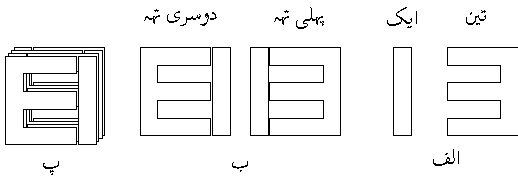
\includegraphics{figTransformersCorePlacement}
\caption{قالبی پتری کے اشکال اور ان کو تہہ در تہہ رکھنے کا طریقہ۔}
\label{شکل_ٹرانسفارم_تہہ_در_تہہ_مرکز}
\end{figure}

ہیجان انگیز برقی رو بے بوجھ اور بوجھ بردار ٹرانسفارمر میں یکساں ہوتا ہے ۔جیسا کہ پہلے بھی ذکر کیا گیا ہے، قوی ٹرانسفارمر اور موٹروں میں برقی دباو اور مقناطیسی بہاو سائن نما ہوتے ہیں جبکہ ہیجان انگیز برقی رو ان میں غیر سائن نما ہوتی ہے لہٰذا اگر
\begin{gather}
\begin{aligned}
\varphi&=\phi_0 \sin \omega t=\phi_0 \cos \left(\omega t -90\degree \right)\\
\hat{\varphi}&=\phi_0 \phase{90\degree}
\end{aligned}
\end{gather}
ہو تو
\begin{gather}
\begin{aligned}\label{مساوات_ٹڑانسفارمر_دباو_سمتیہ}
e_1&=N_1 \frac{\dif \varphi}{\dif t}=\omega N_1 \phi_0 \cos \omega t\\
\hat{E_1}&=\omega N_1 \phi_0 \phase{0}
\end{aligned}
\end{gather}
ہو\حاشیہد{اس مساوات میں اور اس کے بعد پوری کتاب میں امالی برقی دباو کے ساتھ منفی کی علامت نہیں لگائی جائے گی} گی۔یہاں \عددیء{\phi_0} مقناطیسی بہاو کے حیطہ کو ظاہر کرتی ہے،اور \عددیء{\omega} زاویائی تعداد ارتعاش کو یعنی \عددیء{2 \pi f} جہاں \عددیء{f} تعداد ارتعاش ہے جسے ہرٹز \عددیء{\si{\hertz}} میں ناپا جاتا ہے۔\عددیء{\hat{E_1}} اور \عددیء{\hat{\varphi}} کے مابین \عددیء{90^{\circ}} کا زاویہ ہے۔یہ شکل \حوالہ{شکل_ٹرانسفارمر_مرکزی_ضیاع_اور_مقناطیسی_رو} میں دکھایا گیا ہے۔\عددیء{e_1} برقی دباو  کی موثر قیمت \عددیء{E_{rms}}  
\begin{align}
E_{rms}=\frac{\omega N_1 \phi_0}{\sqrt{2}}=4.44 f N_1 \phi_0
\end{align}
ہے۔اس کو ہم یوں بھی لکھ سکتے ہیں
\begin{align}\label{مساوات_ٹرانسفارمر_درکار_ہیجان_بہاو}
\phi_0=\frac{E_{rms}}{4.44 f N_1 \phi_0}
\end{align}

یہاں رکھ کر دوبارہ نظر ثانی کرتے ہیں۔ اگر ایک  لچھے پر \عددیء{E_{rms}} موثر برقی دباو لاگو کی جائے تو یہ لچھا اتنی ہیجان انگیز برقی رو \عددیء{i_{\varphi}} گزرنے دیتی ہے جس سے نمودار ہونے والا مقناطیسی بہاو مساوات \حوالہ{مساوات_ٹرانسفارمر_درکار_ہیجان_بہاو}  میں دیئے گئے مقناطیسی بہاو \عددیء{\phi_0} کے برابر ہو۔ یہ بات نہ صرف ٹرانسفارمر بلکہ کسی بھی مقناطیسی دور کے لئے درست اور لازم ہے۔
\begin{figure}
\centering
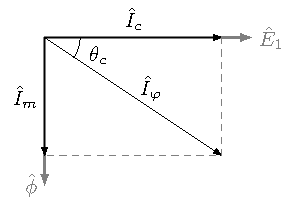
\includegraphics{figTransformersCoreLossAndMagnetizingCurrents}
\caption{مختلف مرحلی سمتیوں کے زاویے۔}
\label{شکل_ٹرانسفارمر_مرکزی_ضیاع_اور_مقناطیسی_رو}
\end{figure}

غیر سائن نما ہیجان انگیز برقی رو \عددیء{\i_{\varphi}} کو \اصطلاح{فوریئر} تسلسل\فرہنگ{فوریئر تسلسل}\حاشیہب{Fourier series}\فرہنگ{Fourier series} سے یوں لکھ سکتے ہیں۔
\begin{align} 
i_{\varphi}=\sum_n {\left( a_n \cos n \omega t + b_n \sin \omega t \right)}
\end{align}
اس میں \عددیء{(a_1 \cos \omega t+b_1 \sin \omega t)} کو \اصطلاح{بنیادی جزو}\فرہنگ{بنیادی جزو}\حاشیہب{fundamental component}\فرہنگ{fundamental component} کہتے ہیں اور باقی حصہ کو  \اصطلاح{موسیقائی جزو}\فرہنگ{موسیقائی جزو}\حاشیہب{harmonic components}\فرہنگ{harmonic components}  کہتے ہیں۔ بنیادی جزو میں \عددیء{a_1 \cos \omega t}، مقناطیسی بہاو سے وجود میں آنے والے امالی برقی دباو \عددیء{e_1} ،  جو کہ مساوات \حوالہ{مساوات_ٹڑانسفارمر_دباو_سمتیہ} میں دی گئی ہے کے ہم قدم ہے۔ یعنی  یہ دونوں وقت کے ساتھ یکساں بڑھتے اور گھٹتے ہیں جبکہ اس میں \عددیء{b_1 \sin \omega t} نوے درجہ زاویہ \عددیء{e_1}  کے پیچھے رہتا ہے۔ قالب میں مختلف وجوہات سے برقی طاقت کی ضائع  کو \عددیء{a_1 \cos \omega t} ظاہر  کرتی ہے۔اسی لئے اس جزو کو \اصطلاح{جزو قالبی ضیاع}\فرہنگ{قالبی ضیاع!جزو}\حاشیہب{core loss component}\فرہنگ{core loss component}  کہتے ہیں۔ہیجان انگیز برقی رو \عددیء{i_{\varphi}} سے اگر \عددیء{a_1 \cos \omega t} منفی کی جائے تو بقایا کو مقناطیس بنانے والا برقی رو\فرہنگ{مقناطیسی برقی رو} یا \اصطلاح{مقناطیسی برقی رو}\حاشیہب{magnetizing current}\فرہنگ{magnetizing current} کہتے ہیں۔ اس  کی تیسری موسیقائی جزو سب سے زیادہ اہم  ہے۔ قوی  ٹرانسفارمروں میں یہ تیسری موسیقائی جزو عموماً  کُل ہیجان انگیز برقی رو  کے \عددیء{40} فی صد ہوتی ہے۔  

سوائے وہاں، جہاں  ہیجان انگیز برقی رو کے اثرات پر غور کیا جا رہا ہو، ہم ہیجان انگیز برقی رو کے غیر سائن نما ہونے کو نظرانداز کرتے ہیں۔ قوی ٹرانسفارمر کی  ہیجان انگیز برقی رو اس کی کُل برقی رو\حاشیہد{کُل برقی رو سے مراد وہ برقی رو ہے جو کُل برقی بوجھ لادنے سے حاصل ہو} کے صرف \عددیء{5}  فی صد کے قریب ہوتی ہے۔ لہٰذا  اس کا اثر بہت کم ہوتا ہے۔ لہٰذا ہم  ہیجان انگیز برقی رو کو سائن نما تصور کر کے اس کے اثرات پر غور کرتے ہیں۔ایسا کرنے سے مسئلہ پر غور کرنا آسان ہو جاتا ہے۔ اس فرضی سائن نما  ہیجان انگیز برقی رو\حاشیہد{یعنی  بدلتی برقی رو \عددیء{i_{\varphi}} کو اب مرحلی سمتیہ کی مدد سے \عددیء{\hat{I_{\varphi}}} لکھتے ہیں} \عددیء{\hat{I_{\varphi}}}  کی موثر قیمت \عددیء{I_{\varphi,rms}} ، اصل  ہیجان انگیز برقی رو کی موثر قیمت کے برابر رکھی جاتی ہے جبکہ اس کا زاویہ \عددیء{\theta_c} یوں رکھا جاتا ہے کہ اس سے حاصل برقی ضیاع اصل برقی ضیاع کے برابر ہو۔ شکل \حوالہ{شکل_ٹرانسفارمر_مرکزی_ضیاع_اور_مقناطیسی_رو}  کی مدد سے یہ بات سمجھنی زیادہ آسان ہے۔ شکل میں اگر دیکھا جائے تو
\begin{align}
p_c=E_{rms} I_{\varphi,rms} \cos \theta_c
\end{align}
جہاں \عددیء{p_c} \اصطلاح{قالبی ضیاع}  ہے۔ لہٰذا  اگر \عددیء{\hat{I_{\varphi}}} اور \عددیء{\hat{E_1}} کے مابین \عددیء{\theta_c} کا زاویہ ہو تو اس سے قالبی ضیاع صحیح حاصل ہوتا ہے۔\عددیء{\hat{I_{\varphi}}} اسی زاویہ  سے  \عددیء{\hat{E_1}}  کے پیچھے رہتا ہے۔

\حصہ{تبادلہ برقی دباو اور تبادلہ برقی رو کے خصوصیات}
ہم شکل \حوالہ{شکل_ٹرانسفارمر_کامل_بار_بردار_ٹرانسفارمر}  کی مدد سے ٹرانسفارمر کا مطالعہ کرتے ہیں۔  ہم فرض کرتے ہیں کہ ابتدائی جانب لچھے کے \عددیء{N_1} اور ثانوی جانب لچھے کے \عددیء{N_2} چکر ہیں اور یہ کہ ان  دونوں لچھوں کی مزاحمت صفر ہے۔ ہم مزید یہ کہتے ہیں کہ پوری مقناطیسی بہاو  قالب ہی میں رہتا ہے اور دونوں لچھوں سے گزرتا ہے۔ قالب میں برقی توانائی ضائع نہیں ہوتی اور اس کی مقناطیسی مستقل اتنی زیادہ ہے کہ ہیجان انگیز برقی رو قابلِ نظر انداز ہے۔ برقی رو \عددیء{i_1}  اور \عددیء{i_2} کی سمتیں یوں رکھی گئی ہیں کہ ان سے وجود میں آنے والے مقناطیسی بہاو ایک دوسرے کی اُلٹ سمتوں میں  ہیں۔ اصل ٹرانسفارمر ان باتوں پر تقریباً پورے اترتے ہیں۔ ایسے ٹرانسفارمر کو کامل ٹرانسفارمر\فرہنگ{ٹرانسفارمر!کامل}\حاشیہب{ideal transformer}\فرہنگ{transformer!ideal}  کہتے ہیں۔
\begin{figure}
\centering
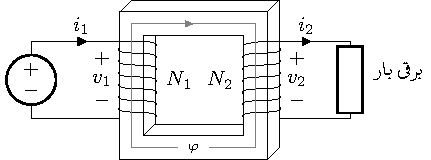
\includegraphics{figTransformersLoadedIdealTransformer}
\caption{کامل بوجھ بردار ٹرانسفارمر۔}
\label{شکل_ٹرانسفارمر_کامل_بار_بردار_ٹرانسفارمر}
\end{figure}

جب اس کامل ٹرانسفارمر کے ابتدائی لچھے پر بدلتی برقی دباو \عددیء{v_1} لاگو کیا جائے تو اس کے قالب میں بدلتا مقناطیسی بہاو  \عددیء{\varphi_m} وجود میں  آئے گا جو ابتدائی لچھے میں   لاگو برقی دباو \عددیء{v_1} کے برابر امالی برقی دباو \عددیء{e_1} کو جنم دے گا۔لہٰذا
\begin{align}
v_1=e_1=N_1 \frac{\dif \varphi_m}{\dif t}
\end{align}
یہ مقناطیسی بہاو دوسرے لچھے سے بھی گزرے گا اور اس میں \عددیء{e_2} امالی برقی دباو کو جنم دے گا جو ثانوی جانب کے سروں پر برقی دباو \عددیء{v_2}  کی صورت میں حاصل ہو گا۔ یعنی
\begin{align}
v_2=e_2=N_2 \frac{\dif \varphi_m}{\dif t}
\end{align}
ان دونوں کی نسبت سے
\begin{align}\label{مساوات_ٹرانسفارمر_تبادلہ_دباو}
\frac{v_1}{v_2}=\frac{N_1 \frac{\dif \varphi_m}{\dif t}}{N_2 \frac{\dif \varphi_m}{\dif t}}=\frac{N_1}{N_2}
\end{align}
لہٰذا ایک کامل ٹرانسفارمر دونوں لچھوں کے چکروں کی نسبت سے \اصطلاح{تبادلہ برقی دباو}\فرہنگ{برقی دباو!تبادلہ}\حاشیہب{voltage transformation}\فرہنگ{voltage!transformation} کرتا ہے۔

چونکہ یہ ایک کامل ٹرانسفارمر ہے لہٰذا اسے جتنی برقی طاقت ابتدائی جانب  دی جائے اتنی ہی برقی طاقت اس سے ثانوی جانب حاصل ہو گی،یعنی
\begin{align}
p=v_1 i_1 = v_2 i_2
\end{align}
یا
\begin{align}
\frac{v_1}{v_2}=\frac{i_2}{i_1}
\end{align}
مساوات  \حوالہ{مساوات_ٹرانسفارمر_تبادلہ_دباو} کی مدد سے
\begin{align}
\frac{v_1}{v_2}=\frac{i_2}{i_1}=\frac{N_1}{N_2}
\end{align}
یہ ایک انتہائی اہم نتیجہ ہے جو ٹرانسفارمر کی تبادلہ برقی دباو اور \اصطلاح{تبادلہ برقی رو}\فرہنگ{برقی رو!تبادلہ}\حاشیہب{current transformation}\فرہنگ{current!transformation}  کی خصوصیات بیان کرتا ہے۔اسے عموماً دو حصوں میں یوں لکھا جاتا ہے۔
\begin{gather}
\begin{aligned}\label{مساوات_ٹرانسفارمر_تبادلہ_دباو_رو}
\frac{v_1}{v_2}&=\frac{N_1}{N_2}\\
\frac{i_1}{i_2}&=\frac{N_2}{N_1}
\end{aligned}
\end{gather}
اس مساوات کی پہلی جزو کہتی ہے کہ ٹرانسفارمر کی دونوں جانب برقی دباو  ان کے چکروں کی راست متناسب  ہو گا جبکہ مساوات کی دوسری جزو کہتی ہے کہ ٹرانسفارمر کے دونوں جانب برقی رو ان کے چکروں کے بالعکس متناسب ہو گا۔

\ابتدا{مثال}
	شکل  \حوالہ{شکل_ٹرانسفارمر_کامل_بار_بردار_ٹرانسفارمر}  میں اگر
\begin{align*}
\hat{V_1}&=220 \phase{0}\\
N_1:N_2&=220:22\\
Z&=R=\SI{10}{\ohm}
\end{align*}
ہوں تو ٹرانسفارمر کی دونوں جانب برقی دباو اور برقی رو معلوم کریں۔

حل:
ابتدائی جانب برقی دباو دیا گیا ہے یعنی \عددیء{220} وولٹ جبکہ ثانوی جانب برقی دباو مساوات \حوالہ{مساوات_ٹرانسفارمر_تبادلہ_دباو_رو} کی پہلی جزو کی مدد سے حاصل کیا جاتا ہے یعنی
\begin{align*}
\hat{V_2}=\frac{N_2}{N_1} \hat{V_1}=\frac{22}{220} \times 220\phase {0}=22\phase{0}
\end{align*}
ثانوی جانب \عددیء{22} وولٹ ہیں جو ابتدائی جانب برقی دباو کے ہم قدم ہے۔ثانوی جانب یہ برقی دباو \عددیء{10} اوہم کی مزاحمت میں برقی رو پیدا کرے گا جسے اوہم کے قانون سے حاصل کیا جاتا ہے یعنی
\begin{align*}
\hat{I_2}=\frac{22 \phase {0}}{10}=2.2\phase {0}
\end{align*}
ثانوی جانب \عددیء{2.2} ایمپیئر برقی رو ہے۔ ابتدائی جانب کی برقی رو مساوات \حوالہ{مساوات_ٹرانسفارمر_تبادلہ_دباو_رو} کی دوسری جزو کی مدد سے حاصل کی جاتی ہے یعنی
\begin{align*}
\hat{I_1}=\frac{N_2}{N_1} \hat{I_2}=\frac{22}{220} \times 2.2\phase{0}=0.22\phase{0}
\end{align*}
\انتہا{مثال}

اس مثال کے نتائج ایک جگہ لکھ کر ان پر غور کرتے ہیں۔
\begin{align*}
\hat{V_1}=220\phase{0}, \quad \hat{V_2}=22\phase{0}, \quad \hat{I_1}=0.22\phase{0}, \quad \hat{I_2}=2.2\phase{0}
\end{align*}
ہم دیکھتے ہیں ابتدائی جانب برقی دباو ثانوی جانب کی برقی دباو کے دس گنا ہے جبکہ برقی رو میں قصہ اُلٹ ہے۔ثانوی جانب کی برقی رو ابتدائی جانب کی برقی رو کے دس گنا ہے۔طاقت دونوں جانب برابر ہے۔یہ نہایت اہم ہے کہ آپ اس بات کو اچھی طرح سمجھ لیں کہ جس جانب برقی دباو زیادہ ہوتا ہے اس جانب برقی رو کم ہوتی ہے۔ لہٰذا زیادہ برقی دباو کی جانب لچھے کے چکر زیادہ ہوں گے اور اس لچھے میں نسبتاً باریک برقی تار استعمال ہو گی جبکہ کم برقی دباو کا لچھا کم چکر کا ہو گا اور اس میں نسبتاً موٹی برقی تار استعمال ہو گی۔ 

\ابتدا{مثال}
	صفحہ \حوالہصفحہ{شکل_ٹرانسفارمر_رکاوٹ_کا_تبادلہ} پر دکھائے گئے شکل \حوالہ{شکل_ٹرانسفارمر_رکاوٹ_کا_تبادلہ}-الف سے رجوع کریں۔ اس شکل میں رکاوٹ \عددیء{Z_2} کو  بدلتی برقی دباو \عددیء{\hat{V_1}} کے ساتھ ایک ٹرانسفارمر کے ذریعہ جوڑا گیا ہے۔اگر
\begin{align*}
\hat{V_1}=110\phase{0},\quad Z_2=R+j X=3+j 2,\quad N_1:N_2=220:22 
\end{align*}
ہوں تو رکاوٹ میں برقی رو اور طاقت کا ضیاع معلوم کریں۔

حل:
	ٹرانسفارمر کی تبادلہ برقی دباو کی خصوصیت سے اس کے ابتدائی جانب \عددیء{110} وولٹ برقی دباو ٹرانسفارمر کی ثانوی جانب تبدیل ہو کر  \عددیء{\hat{V_s}} ہو جائیں گے جہاں
\begin{align*}
\hat{V_s}=\frac{N_2}{N_1} \hat{V_1}=\frac{22}{220} \times 110\phase{0}=11\phase{0}
\end{align*}
ہے لہٰذا
\begin{align*}
\hat{I_2}=\frac{\hat{V_s}}{Z}=\frac{11\phase{0}}{3+j 2}= 3.05\phase{-33.69\degree}
\end{align*}
اور برقی طاقت کا ضیاع \عددیء{p_z}
\begin{align*}
p_z=I_2^2 R=3.05^2 \times 3=\SI{27.9}{\watt}
\end{align*}
\انتہا{مثال}

\حصہ{ثانوی جانب بوجھ کا ابتدائی جانب اثر}\شناخت{حصہ_ٹرانسفارمر_ثانوی_بار_کا_ابتدائی_جانب_اثر}
یہاں صفحہ \حوالہصفحہ{شکل_ٹرانسفارمر_کامل_بار_بردار_ٹرانسفارمر} پر دکھائے گئے  شکل \حوالہ{شکل_ٹرانسفارمر_کامل_بار_بردار_ٹرانسفارمر}  سے رجوع کریں۔ہم حصہ \حوالہ{حصہ_ٹرانسفارمر_امالی_برقی_دباو}  میں دیکھ چکے ہیں کہ اگر ایک بے بوجھ ٹرانسفارمر کی ابتدائی لچھے پر بدلتی برقی دباو \عددیء{v_1} لاگو کی جائے تو اس لچھے میں ہیجان انگیز برقی رو \عددیء{i_{\varphi}} گزرے گی۔اس برقی رو کی مقناطیسی دباو \عددیء{N_1 i_{\varphi}} قالب میں مقناطیسی بہاو \عددیء{\varphi_m}\حاشیہد{\عددیء{\varphi} کو یہاں \عددیء{\varphi_m} کہا گیا ہے۔} کو جنم دے گی ۔اگر لچھے کی مزاحمت صفر ہو تو \عددیء{\varphi_m} ابتدائی لچھے میں \عددیء{e_1} امالی برقی دباو پیدا کرے گی جہاں
\begin{align}\label{مساوات_ٹرانسفارمر_دباو_برابر_بہاو_تفرق}
v_1=e_1=N_1 \frac{\dif \varphi_m}{\dif t}
\end{align}
ہو گی۔

اب ہم ثانوی جانب  برقی بوجھ لادتے ہیں۔ ایسا کرنے سے بوجھ بردار ٹرانسفارمر\فرہنگ{ٹرانسفارمر!بوجھ بردار}\حاشیہب{loaded transformer}  کے  ثانوی جانب  برقی رو \عددیء{i_2} رواں ہو گی جس کی وجہ سے \عددیء{N_2 i_2} مقناطیسی دباو وجود میں آئے گی۔ اس مقناطیسی دباو کی وجہ سے قالب میں مقناطیسی بہاو \عددیء{\varphi_{\textup{بوجھ}}}  پیدا ہو گا۔ اگر اس مقناطیسی بہاو کا کچھ  نہ کیا جائے تو قالب میں پہلے سے موجود مقناطیسی بہاو تبدیل ہو کر \عددیء{\varphi_{\textup{نئی}}=\varphi_{m}-\varphi_{\textup{بوجھ}}} ہو جائے گا اور یوں ابتدائی لچھے میں امالی دباو تبدیل ہو کر \عددیء{e_{\textup{نئی}}} ہو جائے گا۔  لہٰذا ابتدائی جانب پر اب امالی دباو اور اس پر لاگو برقی دباو برابر نہیں ہونگے جو کہ مساوات \حوالہ{مساوات_ٹرانسفارمر_دباو_برابر_بہاو_تفرق}  کی موجودگی میں ناممکن ہے۔ لہٰذا اس مقناطیسی بہاو \عددیء{\varphi_{\textup{بوجھ}}}  کے اثر کو ختم کرنے کیلئے ابتدائی لچھے میں برقی رو \عددیء{i_{1}} نمودار ہو گی جو اس مقناطیسی دباو یعنی \عددیء{N_2 i_2} کے اثر کو ختم کر دے گی یعنی
\begin{align}
N_1 i_1=N_2 i_2
\end{align}
یہ وہ ذریعہ ہے جس سے ابتدائی جانب معلوم ہوتا ہے کہ ثانوی جانب پر بوجھ لدا ہے۔ شکل میں دونوں لچھوں میں برقی رو کی سمتیں یوں ہیں کہ ان کے مقناطیسی بہاو آپس میں اُلٹ سمت میں ہیں لہٰذا  قالب میں اب پھر مقناطیسی بہاو \عددیء{\varphi_m}  کے برابر  ہے جیسا کہ ہونا چاہئے تھا۔ اس مساوات کو یوں لکھ سکتے ہیں
\begin{align}\label{مساوات_ٹرانسفارمر_برقی_رو_اور_چکر_شرح}
\frac{i_1}{i_2}=\frac{N_2}{N_1}
\end{align}
یہ وہی مساوات ہے جو کامل ٹرانسفارمر کے لئے ثابت کی گئی تھی۔
%
\حصہ{ٹرانسفارمر کی علامت پر نقطوں کا مطلب}
	شکل \حوالہ{شکل_ٹرانسفارمر_کامل_بار_بردار_ٹرانسفارمر}  میں ٹرانسفارمر کے لچھوں پر نکتے لگائے گئے ہیں۔ یہ نکتے اس بات کو ظاہر کرتے ہیں کہ اگر ایک طرف کے لچھے پر برقی دباو \عددیء{v_1} یوں ہو کہ نکتے والا سرا مثبت اور بغیر نکتے والا سرا منفی ہو تو دوسرے لچھے  پر برقی دباو \عددیء{v_2} اس طرح ہو گا کہ اس لچھے کا بھی  نکتے والا سرا مثبت اور بغیر نکتے والا سرا منفی ہو گا۔

مزید یہ کہ ابتدائی جانب برقی رو ٹرانسفارمر کے نکتے والے سرے سے ٹرانسفارمر کی اندر جانب ہو گا جبکہ ثانوی جانب برقی رو نقطہ والے سرے سے ٹرانسفارمر سے باہر نکلے گا۔

 یوں  \عددیء{v_1} اور \عددیء{v_2} وقت کے ساتھ یکساں تبدیل ہوتے ہیں اور ان کے مابین صفر زاویہ ہے۔ لہٰذا یہ دو برقی دباو \اصطلاح{ہم قدم}\فرہنگ{ہم قدم}\حاشیہب{in-phase}\فرہنگ{in-phase} ہیں۔

\حصہ{رکاوٹ کا تبادلہ}
اس حصہ میں کامل ٹرانسفارمر میں رکاوٹ کے تبادلہ پر غور کیا جائے گا۔شکل \حوالہ{شکل_ٹرانسفارمر_رکاوٹ_کا_تبادلہ}-الف میں ایک ٹرانسفارمر دکھایا گیا ہے جس کی ابتدائی جانب سائن نما برقی دباو  \عددیء{\hat{V_1}=V_1\phase{\theta}}  لاگو کیا گیا ہے۔یہاں مرحلی سمتیہ استعمال کئے جائیں گے۔

جیسے اُوپر ذِکر ہوا، برقی دباو \عددیء{\hat{V_1}} اور \عددیء{\hat{V_2}} آپس میں ہم قدم ہیں اور  اسی طرح برقی رو \عددیء{\hat{I_1}} اور \عددیء{\hat{I_2}} آپس میں  ہم قدم ہیں۔مساوات \حوالہ{مساوات_ٹرانسفارمر_تبادلہ_دباو} اور  مساوات \حوالہ{مساوات_ٹرانسفارمر_برقی_رو_اور_چکر_شرح}   کو مرحلی سمتیہ کی مدد سے یوں لکھ سکتے ہیں
\begin{gather}
\begin{aligned}
\hat{V_1}&=\left(\frac{N_1}{N_2} \right) \hat{V_2}\\
\hat{I_1}&=\left(\frac{N_2}{N_1} \right) \hat{I_2}
\end{aligned}
\end{gather}
چونکہ رکاوٹ
\begin{align}
Z_2=\frac{\hat{V_2}}{\hat{I_2}}=\abs{Z_2}\phase{\theta_z}
\end{align}
کے برابر ہے لہٰذا
\begin{align}\label{مساوات_ٹرانسفارمر_تبادلہ_رکاوٹ_الف}
\frac{\hat{V_1}}{\hat{I_1}}=\left(\frac{N_1}{N_2} \right)^2 \frac{\hat{V_2}}{\hat{I_2}}=\left(\frac{N_1}{N_2} \right)^2  Z_2
\end{align}
اب اگر ہم ٹرانسفارمر بمع اس پر لدے رکاوٹ  کی جگہ برقی دباو \عددیء{\hat{V_1}} کو رکاوٹ \عددیء{Z_1} پر لاگو کریں جہاں اس رکاوٹ کی قیمت
\begin{align}\label{مساوات_ٹرانسفارمر_متبادل_رکاوٹ_تعریف}
Z_1=\left(\frac{N_1}{N_2} \right)^2  Z_2
\end{align}
ہو تو \عددیء{\hat{V_1}} سے حاصل برقی رو یا اس سے حاصل برقی طاقت تبدیل نہیں ہو گی۔یہ شکل \حوالہ{شکل_ٹرانسفارمر_رکاوٹ_کا_تبادلہ}-ب میں دکھایا گیا ہے جہاں سے واضح ہے کہ
\begin{align}\label{مساوات_ٹرانسفارمر_تبادلہ_رکاوٹ_ب}
\frac{\hat{V_1}}{\hat{I_1}}=Z_1=\left(\frac{N_1}{N_2} \right)^2  Z_2
\end{align}
لہٰذا شکل کے الف اور ب دونوں حصوں سے  برقی دباو \عددیء{\hat{V_1}} کی برقی رو مساوات \حوالہ{مساوات_ٹرانسفارمر_تبادلہ_رکاوٹ_الف}  اور مساوات \حوالہ{مساوات_ٹرانسفارمر_تبادلہ_رکاوٹ_ب}  سے یکساں حاصل ہوتی ہے یعنی
\begin{align}
\hat{I_1}=\frac{\hat{V_1}}{\left(\frac{N_1}{N_2} \right)^2  Z_2}
\end{align}
اور یوں الف اور با  دونوں حصوں میں  برقی دباو \عددیء{\hat{V_1}} سے حاصل برقی طاقت برابر ہے یعنی
\begin{align}
p=\hat{V_1} \cdot \hat{I_1}=\frac{V_1^2 \cos \theta_z}{\left(\frac{N_1}{N_2} \right)^2  \abs{Z_2}}
\end{align}
%
\begin{figure}
\centering
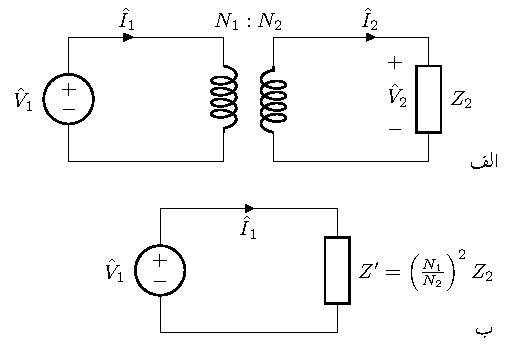
\includegraphics{figTransformersImpedanceTransformation}
\caption{ٹرانسفارمر کی تبادلہ رکاوٹ کی خصوصیت۔}
\label{شکل_ٹرانسفارمر_رکاوٹ_کا_تبادلہ}
\end{figure}
	یوں اگر ٹرانسفارمر کے ثانوی جانب  رکاوٹ \عددیء{Z_2} کا بوجھ ہو تو حساب کرتے وقت ہم یہ اخذ کر سکتے ہیں کہ  ٹرانسفارمر بمع رکاوٹ \عددیء{Z_2} کی  جگہ  صرف  \عددیء{Z_1} رکاوٹ لگی ہے، جہاں \عددیء{Z_1} مساوات \حوالہ{مساوات_ٹرانسفارمر_متبادل_رکاوٹ_تعریف}  سے حاصل ہوتی ہے۔ رکاوٹ کا یوں ٹرانسفارمر کی ایک جانب سے دوسری جانب تبادلہ کیا جاسکتا ہے۔ٹرانسفارمر کی اس خاصیت کو  \اصطلاح{تبادلہ رکاوٹ}\فرہنگ{تبادلہ!رکاوٹ}\حاشیہب{impedance transformation}\فرہنگ{impedance transformation} کی خصوصیت  کہتے ہیں۔
%
\ابتدا{مثال}
شکل \حوالہ{شکل_ٹرانسفارمر_برقی_طاقت_کی_منتقلی}-الف میں رکاوٹ \عددیء{Z_B} کا برقی بوجھ ایک جنریٹر پر لدا ہے۔بوجھ تک برقی طاقت دو برقی تاروں کے ذریعہ منتقل کیا گیا ہے۔ان تاروں کی مجموعہ رکاوٹ \عددیء{Z_t} ہے۔
\begin{figure}
\centering
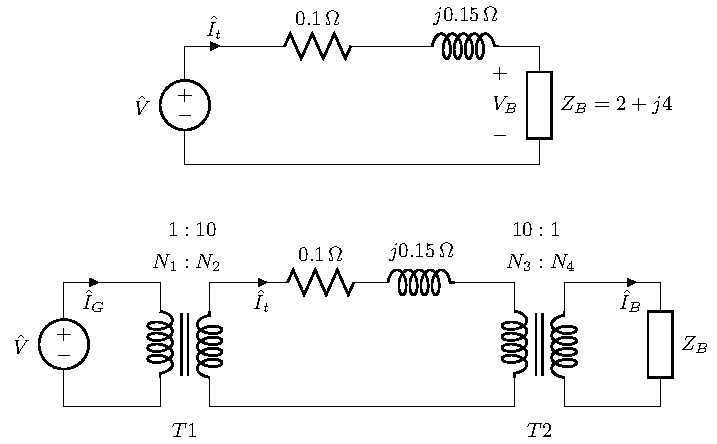
\includegraphics{figTransformersPowerTransmission}
\caption{برقی طاقت کی منتقلی۔}
\label{شکل_ٹرانسفارمر_برقی_طاقت_کی_منتقلی}
\end{figure}
%
\begin{figure}
\centering
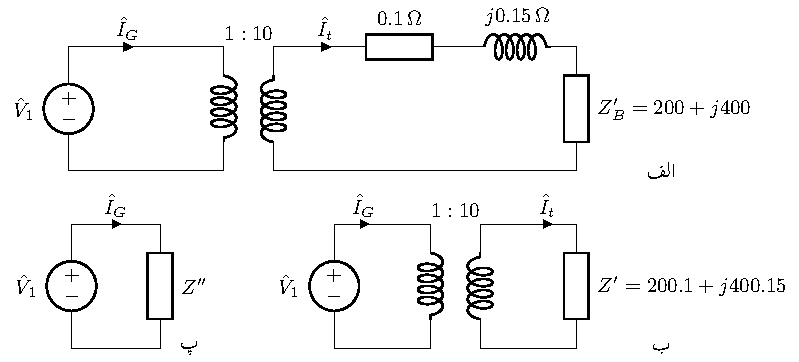
\includegraphics{figTransformersStepByStepSolution}
\caption{ٹرانسفارمر قدم با قدم حل کرنے کا طریقہ۔}
\label{شکل_ٹرانسفارمر_قدم_با_قدم_حل}
\end{figure}

شکل-ب میں جنریٹر کے قریب نسب برقی دباو بڑھانے والا ٹرانسفارمر برقی دباو کو دس گنا بڑھاتا ہے اور برقی بوجھ کے قریب نسب برقی دباو گھٹانے والا ٹرانسفارمر برقی دباو کو دس گنا گھٹاتا ہے۔اس حصہ میں وہی برقی تار استعمال کئے گئے ہیں لہٰذا ان کی بھی مجموعہ رکاوٹ \عددیء{Z_t} ہی ہے۔
اگر 
\begin{align*}
Z_B=2+j 4, \quad Z_t=0.1 +j 0.15, \quad \hat{V}=415\phase{0}
\end{align*}
ہوں تو دونوں صورتوں میں
\begin{itemize}
\item
برقی بوجھ پر برقی دباو معلوم کریں،
\item
برقی تاروں میں برقی طاقت کی ضیاع معلوم کرین۔
\end{itemize}

حل الف:
\begin{align*}
\hat{I_G}=\hat{I_t}=\hat{I_B}&=\frac{\hat{V}}{Z_t+Z_B}=\frac{415\phase{0}}{0.1+j 0.15+2+j 4}\\
&=\frac{415\phase{0}}{2.1+j 4.15}=89.23\phase{-63.159\degree}\\
&=40.3-j79.6
\end{align*}
یوں رکاوٹ پر برقی دباو
\begin{align*}
\hat{V_B}=\hat{I_B} Z_B&=\left(40.3-j79.6 \right) \left( 2+j 4\right)\\
&=399+j2=399\phase{0.287\degree}
\end{align*}
اور برقی تاروں میں برقی طاقت کا ضیاع ہے
\begin{align*}
p_t=I_t^2 R_t=89.23^2 \times 0.1=\SI{796}{\watt}
\end{align*}

حل ب:
شکل \حوالہ{شکل_ٹرانسفارمر_برقی_طاقت_کی_منتقلی} اور شکل \حوالہ{شکل_ٹرانسفارمر_قدم_با_قدم_حل}  سے رجوع کریں۔شکل  \حوالہ{شکل_ٹرانسفارمر_برقی_طاقت_کی_منتقلی} میں ٹرانسفارمر \عددیء{T_2} کے ثانوی جانب رکاوٹ کا مساوات \حوالہ{مساوات_ٹرانسفارمر_متبادل_رکاوٹ_تعریف}  کی مدد سے اس کی ابتدائی جانب تبادلہ سے ملتا ہے
\begin{align*}
Z_B'=Z_1=\left(\frac{N_3}{N_4} \right)^2 Z_B=\left(\frac{10}{1} \right)^2 \left(2+j 4 \right)=200+j 400
\end{align*}
یوں شکل \حوالہ{شکل_ٹرانسفارمر_قدم_با_قدم_حل}-الف حاصل ہوتا ہے۔اس شکل میں اب برقی تار کی رکاوٹ اور  تبادلہ شدہ رکاوٹ سلسلہ وار جُڑے ہیں۔ان کے مجموعہ  کو \عددیء{Z'} کہتے ہوئے
\begin{align*}
Z'=Z_t+Z_B'=0.1+j 0.15+200+j 400=200.1+j400.15
\end{align*}
یہ شکل \حوالہ{شکل_ٹرانسفارمر_قدم_با_قدم_حل}-ب میں دکھایا گیا ہے۔ایک مرتبہ دوبارہ مساوات \حوالہ{مساوات_ٹرانسفارمر_متبادل_رکاوٹ_تعریف}  استعمال کرتے ہوئے
\begin{align*}
Z''=\left(\frac{N_1}{N_2} \right)^2 Z'=\left(\frac{1}{10} \right)^2 \left(200.1+j400.15 \right)=2.001+j4.0015
\end{align*}
شکل \حوالہ{شکل_ٹرانسفارمر_قدم_با_قدم_حل}-پ میں دکھایا گیا ہے۔اب
\begin{align*}
\hat{I_G}=\frac{\hat{V}}{Z''}=\frac{415\phase{0}}{2.001+j4.0015}=92.76\phase{-63.432\degree}
\end{align*}
یہاں سے شکل \حوالہ{شکل_ٹرانسفارمر_قدم_با_قدم_حل}-ب  کی مدد سے اگر جنریٹر کی برقی رو معلوم ہو تو تبادلہ برقی رو سے
\begin{align*}
\hat{I_t}=\left(\frac{N_1}{N_2} \right) \hat{I_G}=\left(\frac{1}{10}\right) 92.76\phase{-63.432\degree}=9.276\phase{-63.432\degree}
\end{align*}
اس سے برقی تار میں طاقت کا ضیاع
\begin{align*}
p_t=I_t^2 R_t=9.276^2  \times 0.1=\SI{8.6}{\watt}
\end{align*}
اسی طرح شکل \حوالہ{شکل_ٹرانسفارمر_برقی_طاقت_کی_منتقلی}  میں اگر \عددیء{\hat{I_t}} معلوم ہو تو تبادلہ برقی رو سے
\begin{align*}
\hat{I_B}&=\left(\frac{N_3}{N_4}\right) \hat{I_t}=\left(\frac{10}{1}\right) 9.276\phase{-63.432\degree}\\
&=92.76\phase{-63.432\degree}=41.5-j 82.9
\end{align*}
اور رکاوٹ پر برقی دباو
\begin{align*}
\hat{V_B}=\hat{I_B} Z_B=\left(41.5-j 82.9 \right) \left(2+j 4 \right)=414+j 0.2
\end{align*}
ہو گی۔

ٹرانسفارمر کے بغیر برقی طاقت کی منتقلی میں برقی تاروں میں طاقت کی ضیاع \عددیء{796} واٹ ہے جبکہ ٹرانسفارمر کے استعمال سے یہ صرف \عددیء{8.6} واٹ ہے یعنی \عددیء{92} گنا کم۔یہی ٹرانسفارمر کی نہایت مقبولیت کی وجہ ہے۔ 
\انتہا{مثال}
%
\حصہ{ٹرانسفارمر کے وولٹ-ایمپیئر}
ٹرانسفارمر کی دونوں جانب برقی دباو ان لچھوں کے چکر پر منحصر ہوتا ہے۔ٹرانسفارمر ایک خاص برقی دباو اور برقی رو کے لئے بنائے جاتے ہیں۔ٹرانسفارمر جس برقی دباو \عددیء{V_1:V_2} کے لئے بنائے جائیں یہ اس سے کم برقی دباو پر بھی استعمال کئے جا سکتے ہیں اگرچہ یہ عموماً بنائے گئے برقی دباو پر ہی چلائے جاتے ہیں۔اسی طرح ٹرانسفارمر جتنی برقی رو \عددیء{I_1:I_2} کے لئے بنائے جائیں انہیں اس سے کم برقی رو پر استعمال کیا جا سکتا ہے۔حقیقت میں عموماً ٹرانسفارمر سے حاصل برقی رو اس حد سے کم ہی رکھی جاتی ہے۔

ٹرانسفارمر کی ایک جانب کی برقی دباو اور برقی رو کا حاصل ضرب اس کی دوسری جانب کی برقی دباو اور برقی رو کے حاصل ضرب کے برابر ہوتا ہے یعنی
\begin{align}
V_1 I_1=V_2 I_2
\end{align}
برقی دباو اور برقی رو کے حاصلِ ضرب  یعنی \عددیء{V_1 I_1} یا \عددیء{V_2 I_2} کو ٹرانسفارمر کی وولٹ ضربِ ایمپیئر کہتے ہیں جسے عموماً چھوٹا کر کے صرف \اصطلاح{وولٹ-ایمپیئر}\فرہنگ{وولٹ-ایمپیئر}
\حاشیہب{volt-ampere, VA}\فرہنگ{volt-ampere}\فرہنگ{VA}  کہا جاتا ہے\حاشیہد{وولٹ-ایمپیئر کو عموماً کلو وولٹ-ایمپیئر یعنی \عددیء{\si{\kilo \volt \ampere}} میں بیان کیا جاتا ہے}۔یہ ٹرانسفارمر کی برقی سکت کی ناپ ہے جو اس پر لگی تختی پر لکھا جاتا ہے۔اس تختی پر ٹرانسفارمر کے برقی دباو اور برقی تعداد ارتعاش بھی لکھے جاتے ہیں۔یوں ٹرانسفارمر کے وولٹ-ایمپیئر
\begin{align}\label{مساوات_ٹرانسفارمر_وولٹ_ایمپئیر}
\textup{وولٹ-ایمپیئر}= V_1 I_1 = V_2 I_2
\end{align}
ہوں گے۔

اگرچہ یہاں ذکر ٹرانسفارمر کا ہو رہا ہے دراصل برقی مشین یعنی موٹر اور جنریٹر کی تختیوں پر بھی ان کے چالو حالت کے برقی دباو، ان کے وولٹ-ایمپیئر اور برقی تعداد ارتعاش لکھے جاتے ہیں۔اس کی وجہ یہ ہے کہ ان سب مشین کی کارکردگی کے بنیادی اصول ایک ہی طرح کے ہیں۔

\ابتدا{مثال}
ایک \عددیء{25000 } وولٹ-ایمپیئر اور \عددیء{11000:220} وولٹ برقی سکت  کے ٹرانسفارمر کے زیادہ برقی دباو کی جانب \عددیء{11000} وولٹ لاگو ہیں۔
\begin{itemize}
\item
اس کی ثانوی جانب زیادہ سے زیادہ کتنی برقی بوجھ ڈالی جا سکتی ہے۔
\item
اس زیادہ سے زیادہ برقی بوجھ پر اس کے ابتدائی لچھے میں برقی رو حاصل کریں۔
\end{itemize}

حل:	اس ٹرانسفارمر کی معلومات یہ ہیں
\begin{align*}
\SI{25}{\kilo \volt \ampere}, \quad 11000:220\,\textup{V}
\end{align*}
اس کی ثانوی جانب برقی دباو تبادلہ برقی دباو کی مساوات سے  \عددیء{220 } وولٹ حاصل ہوتا ہے۔یوں اس کی ثانوی جانب یعنی کم برقی دباو کی جانب زیادہ سے زیادہ برقی رو مساوات \حوالہ{مساوات_ٹرانسفارمر_وولٹ_ایمپئیر}  سے حاصل کیا جاتا ہے۔
\begin{align*}
I_2=\frac{25000}{220}=\SI{113.636}{\ampere}
\end{align*}
اسی طرح اس کی ابتدائی جانب زیادہ سے زیادہ برقی رو اسی مساوات سے یوں حاصل ہوتی ہے
\begin{align*}
I_1=\frac{25000}{11000}=\SI{2.27}{\ampere}
\end{align*}
\انتہا{مثال}
%
ٹرانسفارمر کی دونوں جانب لچھوں میں استعمال برقی تار کی موٹائی یوں رکھی جاتی ہے کہ ان میں کثافتِ برقی رو \عددیء{J}\حاشیہد{\عددیء{\SI{1000}{\kilo \volt \ampere}}  ٹرانسفارمر کی لچھوں میں کثافتِ برقی رو تقریباً  \عددیء{\SI{3}{\ampere / \milli \meter \squared}} رکھی جاتی ہے} یکساں ہو۔لچھوں کی مزاحمت میں برقی رو گزرنے سے برقی طاقت کا ضیاع ہوتا ہے جس سے یہ گرم ہوتے ہیں۔ٹرانسفارمر کی برقی رو کی حد لچھوں کی گرمائش پر منحصر ہوتی ہے۔ان کی زیادہ سے زیادہ حرارت کو محفوظ حد کے اندر رکھا جاتا ہے۔

بڑے ٹرانسفارمر کے قالب اور لچھے ایک غیر موصل تیل سے بھری ٹینکی میں ڈبوئے رکھے جاتے ہیں۔یہ تیل ایک تو برقی لچھوں کی حرارت کم کرنے میں مدد دیتا ہے اور دوسری جانب غیر موصل ہونے کی وجہ سے یہ زیادہ برقی دباو کے حصوں کو برقی طور پر جدا رکھنے میں مدد دیتا ہے۔یہ تیل تقریباً  \عددیء{\SI{80}{\celsius}} پر خراب ہونا شروع ہو جاتا ہے اور ہر \عددیء{\SI{8}{\celsius}} اضافی درجہ حرارت پر اس کی زندگی آدھی ہوتی رہتی ہے۔یعنی اگر \عددیء{\SI{80}{\celsius}} پر تیل کی کارآمد زندگی \عددیء{x} سال ہے تو \عددیء{\SI{88}{\celsius}} پر \عددیء{x/2} سال اور  \عددیء{\SI{96}{\celsius}} پر یہ صرف  \عددیء{x/4} سال ہو گی۔

	ٹرانسفارمر جس برقی دباو کے لئے بنایا جائے  یہ اس پر لگی تختی پر لکھا جاتا ہے۔اس سے حاصل برقی رو کی حد کو ایک مختلف طریقے سے لکھا جاتا ہے۔

\حصہ{ٹرانسفارمر کے امالہ اور اس کے مساوی دور}
\جزوحصہ{لچھے کی مزاحمت اور اس کی متعاملہ علیحدہ کرنا}
ٹرانسفارمر کی ابتدائی لچھے کی مزاحمت \عددیء{R_1} کو ہم نے حصہ \حوالہ{حصہ_ٹرانسفارمر_امالی_برقی_دباو} مساوات \حوالہ{مساوات_ٹرانسفارمر_بیرونی_اندرونی_دباو_فرق} میں دیکھا۔لچھے کی مزاحمت کو لچھے سے باہر لچھے کے ساتھ سلسلہ وار جڑا دکھایا گیا تھا۔دیکھتے ہیں یہ کیسے ممکن ہوتا ہے۔

شکل \حوالہ{شکل_ٹرانسفارمر_لچھے_کی_مزاحمت_اور_متعاملہ}-الف میں ایک لچھے پر بدلتی برقی دباو لاگو کا گیا ہے۔اگر لچھے کی برقی تار کو نہایت چھوٹے ٹکڑوں میں تقسیم کیا جائے تو اس کے ہر ٹکڑے کی نہایت کم مزاحمت  اور متعاملہ ہو گی۔ایسا ایک ٹکڑا شکل-ب میں دکھایا گیا ہے۔چونکہ لچھا ان سب ٹکڑوں کے سلسلہ وار جڑنے سے بنا ہے  لہٰذا شکل-الف کو ہم شکل-پ کی طرح بنا سکتے ہیں جہاں لچھے کے \عددیء{n} ٹکڑے  کیے گیے ہیں۔
\begin{figure}
\centering
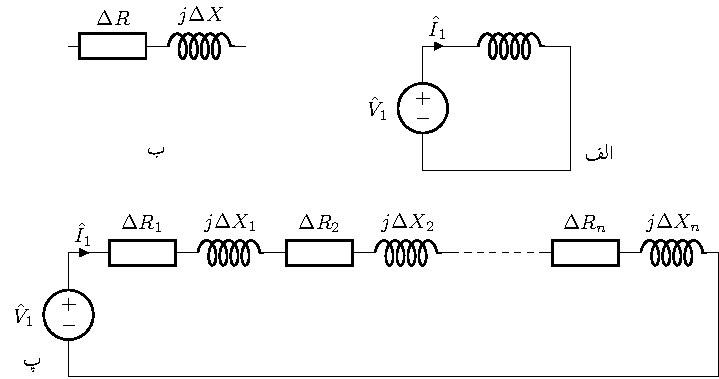
\includegraphics{figTransformersCoilResistanceAndReactance}
\caption{لچھے کی مزاحمت اور متعاملہ۔}
\label{شکل_ٹرانسفارمر_لچھے_کی_مزاحمت_اور_متعاملہ}
\end{figure}

اس دور کی مساوات لکھ کر حل کرتے ہیں۔
\begin{align*}
\hat{V}_1&=\hat{I}_1 \left(\Delta R_1 + j \Delta X_1 +\Delta R_2 + j \Delta X_2 + \cdots \Delta R_n + j \Delta X_n   \right)\\
&=\hat{I}_1 \left(\Delta R_1 +\Delta R_2 +\cdots \Delta R_n   \right)+\hat{I}_1 \left(j \Delta X_1 + j \Delta X_2+\cdots   j \Delta X_n   \right)\\
&=\hat{I}_1 \left( R +j X \right)
\end{align*}
جہاں
\begin{align*}
R&=\Delta R_1 +\Delta R_2 +\cdots \Delta R_n\\
X&=\Delta X_1 + \Delta X_2 +\cdots   \Delta X_n
\end{align*}
اس سے  شکل \حوالہ{شکل_ٹرانسفارمر_لچھے_کی_مزاحمت_اور_متعاملہ_کی_علیحدگی}  حاصل ہوتا ہے  جس سے  ثابت ہوتا ہے کہ حساب کتاب کی غرض سے لچھے کی مزاحمت اور متعاملہ علیحدہ کیے جا سکتے ہیں۔
\begin{figure}
\centering
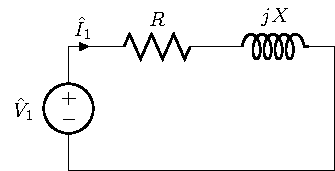
\includegraphics{figTransformersCoilResistanceAndReactanceSeparation}
\caption{لچھے کی مزاحمت اور متعاملہ کی علیحدگی۔}
\label{شکل_ٹرانسفارمر_لچھے_کی_مزاحمت_اور_متعاملہ_کی_علیحدگی}
\end{figure}
%
\جزوحصہ{رِستا امالہ}
اوپر ایک کامل ٹرانسفارمر زیرِ بحث رہا۔ اب ہم ٹرانسفارمر میں ان عناصر کا ذکر کرتے ہیں جن کی وجہ سے ٹرانسفارمر غیر کامل ہو جاتا ہے۔ بہت سی جگہوں پر ٹرانسفارمر استعمال کرتے وقت ان عناصر کو مدِ نظر رکھ کر ہی اس کا صحیح استعمال ممکن ہوتا ہے۔ ان عناصر کے اثر کو شامل کرنے کے لئے ہم  ٹرانسفارمر کا مساوی دور بناتے ہیں۔

ابتدائی لچھے کے مقناطیسی بہاو کو دو حصوں میں تقسیم کیا جا سکتا ہے۔ پہلا حصہ وہ جو قالب سے گزر کر ابتدائی اور ثانوی لچھے دونوں سے گزرتا ہے۔ یہ ان کا مشترکہ مقناطیسی بہاو ہے اور دوسرا حصہ وہ جو صرف ابتدائی لچھے سے گزرتا ہے اور زیادہ تر قالب کے باہر خلاء میں ہی رہتا ہے۔  اس کو \اصطلاح{رستا  مقناطیسی بہاو}\فرہنگ{مقناطیسی بہاو!رستا}\حاشیہب{leakage magnetic flux}\فرہنگ{magnetic flux!leakage}   کہتے ہیں۔ یہ شکل میں دکھایا گیا ہے۔ چونکہ ہوا میں مقناطیسی مستقل \عددیء{\mu_0} مقررہ ہے لہٰذا یہاں ہچکچاہٹ بھی مقررہ ہے۔  یوں رستا مقناطیسی بہاو ابتدائی لچھے کی برقی رو کے  براہ راست متناسب ہوتی ہے۔

 اس کے اثر کو بالکل لچھے کی مزاحمت کی طرح لچھے سے باہر \اصطلاح{رستا امالہ}\فرہنگ{رستا!امالہ}\حاشیہب{leakage inductance}\فرہنگ{leakage inductance} \عددیء{L_1} یا \اصطلاح{رستا متعاملہ}\فرہنگ{رستا!متعاملہ}\حاشیہب{leakage reactance}\فرہنگ{leakage reactance}  \عددیء{X_1=2\pi f L_1} سے ظاہر کیا جاتا ہے۔

ٹرانسفارمر کے ابتدائی لچھے میں برقی رو \عددیء{\hat{I_1}}  گزرنے سے رستا متعاملہ میں \عددیء{\hat{V}_{X1}=j \hat{I}_1 X_1} برقی دباو اور لچھے کے تار کی مزاحمت \عددیء{R_1} میں
 \عددیء{\hat{V}_{R1}=\hat{I}_1 R_1} برقی دباو گھٹتا ہے۔

یوں ابتدائی لچھے  پر لاگو برقی دباو \عددیء{\hat{V}_1} میں سے کچھ برقی دباو \عددیء{R_1} میں کم ہو گا،  کچھ  متعاملہ \عددیء{X_1} میں کم ہو گا اور بقایا  \عددیء{\hat{E}_1} کے برابر ہو گا۔  یہ شکل \حوالہ{شکل_ٹرانسفارمر_ماڈل_حصہ_اول}  میں دکھایا گیا ہے۔
\begin{figure}
\centering
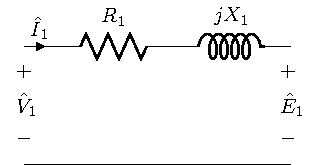
\includegraphics{figTransformersModelFirstPart}
\caption{ٹرانسفارمر مساوی دور، حصہ اول۔}
\label{شکل_ٹرانسفارمر_ماڈل_حصہ_اول}
\end{figure}
%

\جزوحصہ{ثانوی برقی رو اور قالب کے اثرات}
قالب میں دونوں لچھوں کا مشترکہ مقناطیسی بہاو ان کے مجموعی مقناطیسی دباو کی وجہ سے وجود میں آتا ہے۔ البتہ اگر ہم کچھ یوں سوچیں تو یہ زیادہ بہتر ہو گا۔ ہم کہتے ہیں کہ ابتدائی برقی رو کو دو شرائط پوری کرنی ہونگی۔ پہلی یہ کہ اسے قالب میں ہیجانی مقناطیسی بہاو وجود میں لانا ہو گا اور دوسری یہ کہ اسے ثانوی لچھے کے پیدا کردہ مقناطیسی بہاو کو ختم کرنا ہو گا۔ لہٰذا ابتدائی برقی رو کو ہم دو حصوں میں تقسیم کر سکتے ہیں۔ ایک حصہ \عددیء{i_{\varphi}} جو ہیجانی مقناطیسی بہاو پیدا کرے اور دوسرا \عددیء{\hat{I}_2'} جو ثانوی لچھے کے مقناطیسی دباو کے اثر کو ختم کرے۔ لہٰذا
\begin{align}
\hat{I}_2'=\frac{N_2}{N_1} \hat{I}_2
\end{align}
	اس باب کے حصہ \حوالہ{حصہ_ٹرانسفارمر_ثانوی_بار_کا_ابتدائی_جانب_اثر}  میں اس پر تفصیل سے غور کیا گیا ہے۔ برقی رو \عددیء{i_{\varphi}} غیر سائن نما ہوتی ہے لیکن پھر بھی  ہم اسے سائن نما\حاشیہد{سائن نما برقی رو کو مرحلی سمتیہ سے ظاہر کیا جاتا ہے} \عددیء{\hat{I}_\varphi}  ہی تصور کرتے ہیں۔ اس کو ہم دو حصوں میں تقسیم کر سکتے ہیں یعنی
\begin{align}\label{مساوات_ٹرانسفارمر_رو_ہیجان_ضیاع_اجزاع}
\hat{I}_\varphi=\hat{I}_c+\hat{I}_m
\end{align}
جہاں \عددیء{\hat{I}_c} اس کا وہ حصہ ہے جو ابتدائی لچھے کی امالی برقی دباو \عددیء{\hat{E}_1} کے ہم قدم ہے اور یہ قالب میں برقی توانائی کے ضیاع کو ظاہر کرتا ہے جبکہ \عددیء{\hat{I}_m} اس کا وہ حصہ ہے جو \عددیء{\hat{E}_1} سے نوے درجہ زاویہ \اصطلاح{پیچھے}\فرہنگ{پیچھے}\حاشیہب{lagging}  ہے اور  لچھے میں مقناطیسی بہاو کو جنم دیتا ہے۔ برقی رو کے ان حصوں کو ہم  ایک مزاحمت \عددیء{R_c}  اور ایک \عددیء{j X_m} سے پیش کرتے ہیں۔ یہ شکل میں دکھایا گیا ہے۔\عددیء{R_c} کی مقدار اتنی رکھی جاتی ہے کہ اس میں برقی طاقت کا ضیاع اصل قالبی ضیاع کے برابر ہو یعنی \عددیء{p_c=E_{1,rms}^2/R_c} ، اسی طرح \عددیء{j X_m} کی مقدار اتنی رکھی جاتی ہے کہ \عددیء{\hat{I}_m=\hat{E}_1/jX_{m}} ہو۔ان دونوں،  یعنی \عددیء{R_c} اور \عددیء{j X_m} ، کی مقدار اصل برقی دباو اور تعدد پر حاصل کئے جاتے ہیں۔ یہ شکل \حوالہ{شکل_ٹرانسفارمر_ماڈل_حصہ_دوم}  میں دکھایا گیا ہے۔

\begin{figure}
\centering
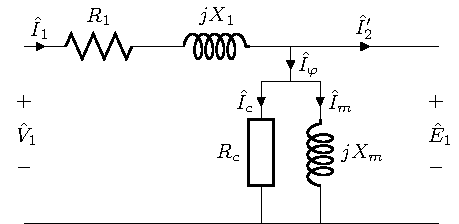
\includegraphics{figTransformersModelSecondPart}
\caption{ٹرانسفارمر مساوی دور، حصہ دوم۔}
\label{شکل_ٹرانسفارمر_ماڈل_حصہ_دوم}
\end{figure}

\جزوحصہ{ثانوی لچھے کی امالی برقی دباو}
قالب میں مشترکہ مقناطیسی بہاو ثانوی لچھے میں امالی برقی دباو \عددیء{\hat{E}_2} پیدا کرے گی اور چونکہ یہی مقناطیسی بہاو ابتدائی لچھے میں \عددیء{\hat{E}_1}  امالی پیدا کرتی ہے لہٰذا
\begin{align}\label{مساوات_ٹرانسفارمر_دباو_رو_شرح}
\frac{\hat{E}_1}{\hat{E}_2}=\frac{N_1}{N_2}
\end{align}
مساوات \حوالہ{مساوات_ٹرانسفارمر_رو_ہیجان_ضیاع_اجزاع} اور مساوات \حوالہ{مساوات_ٹرانسفارمر_دباو_رو_شرح}  کو ایک کامل ٹرانسفارمر سے ظاہر کیا جا سکتا ہے۔ یہ شکل \حوالہ{شکل_ٹرانسفارمر_ماڈل_حصہ_ثوم}  میں دکھایا گیا ہے۔
\begin{figure}
\centering
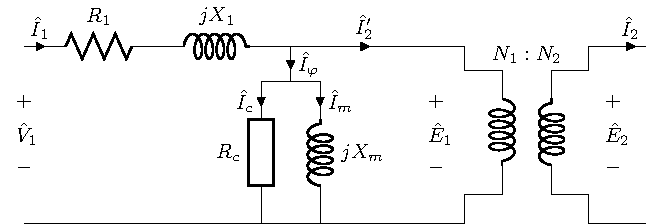
\includegraphics{figTransformersModelThirdPart}
\caption{ٹرانسفارمر مساوی دور، حصہ ثوم۔}
\label{شکل_ٹرانسفارمر_ماڈل_حصہ_ثوم}
\end{figure}

\جزوحصہ{ثانوی لچھے کی مزاحمت اور متعاملہ کے اثرات}
ثانوی لچھے کے سروں پر البتہ  \عددیء{\hat{E}_2} برقی دباو نہیں ہو گا چونکہ ثانوی لچھے کے، بالکل ابتدائی لچھے کی طرح، مزاحمت \عددیء{R_2}  اور متعاملہ  \عددیء{j X_2} ہوں گے جن میں ثانوی برقی رو \عددیء{\hat{I}_2}  کی وجہ سے برقی دباو گھٹے گا۔  لہٰذا ثانوی لچھے کے سروں پر برقی دباو \عددی{\hat{V}_2} قدرِ کم ہو گا۔ یعنی
\begin{align}
\hat{V}_2=\hat{E}_2-\hat{I}_2 R_2-j \hat{I}_2 X_2
\end{align}
	یوں حاصل ٹرانسفارمر کا مکمل مساوی دور یا \اصطلاح{ریاضی نمونہ}\فرہنگ{ریاضی نمونہ}\حاشیہب{mathematical model}\فرہنگ{model} شکل  \حوالہ{شکل_ٹرانسفارمر_مکمل_ماڈل} میں دکھایا گیا ہے۔
\begin{figure}
\centering
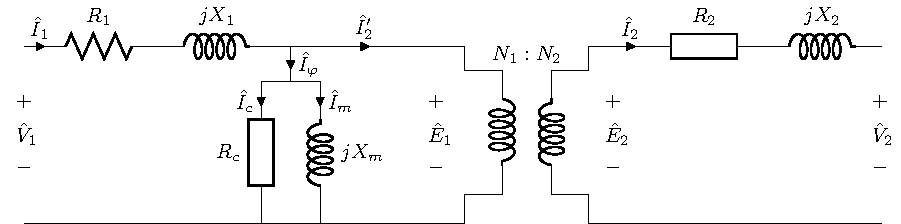
\includegraphics[width=0.9\linewidth]{figTransformersModelComplete}
\caption{ٹرانسفارمر کا مکمل مساوی دور یا ریاضی نمونہ۔}
\label{شکل_ٹرانسفارمر_مکمل_ماڈل}
\end{figure}

\جزوحصہ{رکاوٹ کا ابتدائی یا ثانوی جانب تبادلہ}
شکل \حوالہ{شکل_ٹرانسفارمر_مکمل_ماڈل}  میں دکھائے دور کے سب جزو کا تبادلہ ایک جانب سے دوسری جانب کیا جا سکتا ہے۔ یہ کرنے سے کامل ٹرانسفارمر کو مساوی دور کی بائیں یا دائیں جانب لے جایا جا سکتا ہے۔شکل \حوالہ{شکل_ٹرانسفارمر_مکمل_ماڈل_ابتدائی_جانب}   میں ثانوی جانب کی رکاوٹ کا ابتدائی جانب تبادلہ کیا گیا ہے جبکہ شکل  \حوالہ{شکل_ٹرانسفارمر_مکمل_ماڈل_ثانوی_جانب}  میں ابتدائی جانب کی رکاوٹ کا ثانوی جانب تبادلہ کیا گیا ہے۔اس طرح حاصل مساوی دور میں عموماً کامل ٹرانسفارمر بنایا ہی نہیں جاتا۔یہی شکل \حوالہ{شکل_ٹرانسفارمر_مکمل_ماڈل_ثانوی_جانب}   میں کیا گیا ہے۔

تبادلہ شدہ رکاوٹ  \عددیء{Z} کو \عددیء{Z'}  سے ظاہر کیا جاتا ہے۔یوں \عددیء{R_2} کے ٹرانسفارمر کی دوسری جانب تبادلہ کے بعد اسے \عددیء{R_2'} سے ظاہر کیا گیا ہے۔

ایسا دور استعمال کرتے وقت یہ ذہن میں رکھنا ہوتا ہے کہ ٹرانسفارمر کے کس جانب دور حل کیا جا رہا ہے۔
\begin{figure}
\centering
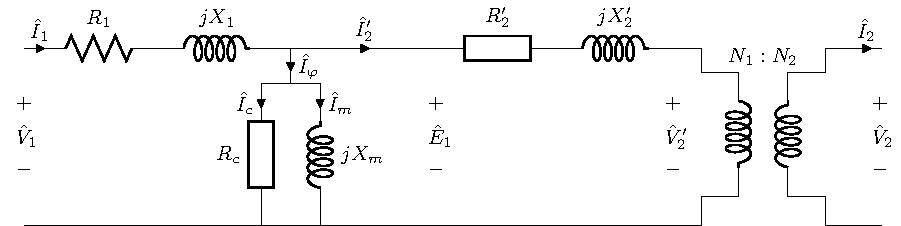
\includegraphics[width=0.9\linewidth]{figTransformersModelShiftedToPrimarySide}
\caption{ثانوی جانب رکاوٹ کا ابتدائی جانب تبادلہ کیا گیا ہے۔}
\label{شکل_ٹرانسفارمر_مکمل_ماڈل_ابتدائی_جانب}
\end{figure}
%
\begin{figure}
\centering
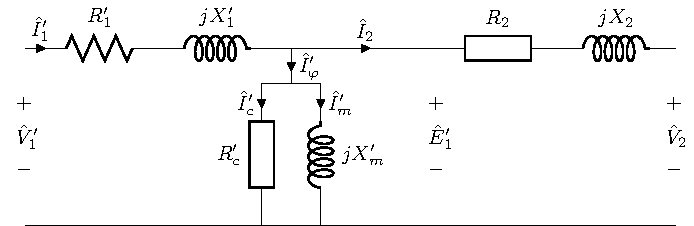
\includegraphics[width=0.9\linewidth]{figTransformersModelShiftedToSecondarySide}
\caption{ابتدائی جانب رکاوٹ کا ثانوی جانب تبادلہ کیا گیا ہے۔}
\label{شکل_ٹرانسفارمر_مکمل_ماڈل_ثانوی_جانب}
\end{figure}


%
\ابتدا{مثال}
ایک \عددیء{50} کلو وولٹ-ایمپیئر اور  \عددیء{2200:220} وولٹ برقی سکت کے ٹرانسفارمر کی زیادہ برقی دباو کی جانب کی رستا رکاوٹ \عددیء{Z_1=0.9+j 1.2}  اوہم اور کم برقی دباو کی جانب کی رِستا رکاوٹ \عددیء{Z_2=0.0089+j 0.011} اوہم ہے۔اگر اس کی \عددیء{R_c=\SI{6.4}{\kilo\ohm}} اور \عددیء{X_m=\SI{47}{\kilo\ohm}}  ہو تو اس کی شکل \حوالہ{شکل_ٹرانسفارمر_مکمل_ماڈل_ابتدائی_جانب}  اور شکل \حوالہ{شکل_ٹرانسفارمر_مکمل_ماڈل_ثانوی_جانب}  میں استعمال ہونے والے جزو معلوم کریں۔

	حل حصہ اول:
معلومات:
\begin{align*}
\SI{50}{\kilo \volt \ampere}, \quad \SI{50}{\hertz}, \quad 2200:220\,\textup{V}
\end{align*}
ٹرانسفارمر کے دونوں جانب کی برقی دباو لچھوں کے چکروں کی نسبت سے ہوتے ہیں لہٰذا
\begin{align*}
\frac{N_1}{N_2}=\frac{2200}{220}=\frac{10}{1}
\end{align*}
یوں اگر ٹرانسفارمر کی رکاوٹ کا زیادہ برقی دباو کی جانب تبادلہ کیا جائے تو
\begin{align*}
R_2'+j X_2' &=\left(\frac{N_1}{N_2} \right)^2 \left(R_2+j X_2 \right)\\
&=\left(\frac{10}{1} \right)^2 \left(0.0089+j 0.011 \right)\\
&=0.89+j 1.1
\end{align*}
جبکہ اس کی بقایا رکاوٹ وہی رہیں گے۔یوں شکل \حوالہ{شکل_ٹرانسفارمر_مکمل_ماڈل_ابتدائی_جانب}  کے جزو حاصل ہوئے۔

	حل حصہ دوم:
اگر مساوی دور کی رکاوٹ کا کم برقی دباو کی جانب تبادلہ کیا جائے تب
\begin{align*}
R_1'+j X_1' &=\left(\frac{N_2}{N_1} \right)^2 \left(R_1+j X_1 \right)\\
&=\left(\frac{1}{10} \right)^2 \left(0.9+j1.2 \right)\\
&=0.009+j0.012
\end{align*}
اسی طرح
\begin{align*}
R_c'&=\left(\frac{N_2}{N_1} \right)^2 R_c=64\\
X_m'&=\left(\frac{N_2}{N_1} \right)^2 X_m=470
\end{align*}
جبکہ \عددیء{Z_2} وہی رہے گا۔
\انتہا{مثال}
%
\جزوحصہ{ٹرانسفارمر کے سادہ ترین مساوی دور}
ایک انجنیئر کو جب ایک ٹرانسفارمر استعمال کرنا ہو تو وہ حساب کرتے وقت شکل \حوالہ{شکل_ٹرانسفارمر_مکمل_ماڈل_ابتدائی_جانب}  میں دیئے گئے دور کو استعمال کر سکتا ہے۔ یہ دور حقیقی ٹرانسفارمر کی بہت اچھی عکاسی کرتا ہے۔ البتہ جہاں ہمیں نہایت صحیح جواب مطلوب نہ ہوں وہاں اس دور کی سادہ اشکال بھی استعمال کی جا سکتیں ہیں۔ اس باب میں ہم ایسے ہی سادہ مساوی دوروں کا ذکر کریں گے۔
\begin{figure}
\centering
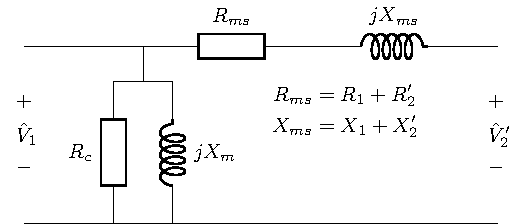
\includegraphics[width=0.9\linewidth]{figTransformersModelLeftHand}
\caption{\عددیء{R_c} اور \عددیء{jX_m} کو بائیں جانب منتقل کیا گیا ہے۔}
\label{شکل_ٹرانسفارمر_بائیں_جانب}
\end{figure}
%
\begin{figure}
\centering
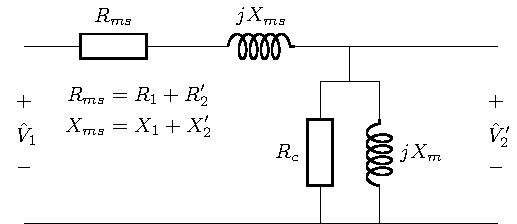
\includegraphics[width=0.9\linewidth]{figTransformersModelRightHand}
\caption{\عددیء{R_c} اور \عددیء{jX_m} کو دائیں جانب منتقل کیا گیا ہے۔}
\label{شکل_ٹرانسفارمر_دائیں_جانب}
\end{figure}

شکل  \حوالہ{شکل_ٹرانسفارمر_مکمل_ماڈل_ابتدائی_جانب} میں \عددیء{R_c} اور \عددیء{X_m} کو بائیں یا دائیں طرف لے جانے سے  شکل  \حوالہ{شکل_ٹرانسفارمر_بائیں_جانب}  اور  شکل \حوالہ{شکل_ٹرانسفارمر_دائیں_جانب}  حاصل ہوتے ہیں۔چونکہ \عددیء{\hat{I}_\varphi} کی مقدار نہایت کم\حاشیہد{\عددیء{\hat{I}_\varphi} ٹرانسفارمر کے کُل برقی بوجھ کے صرف دو سے چھ فی صد ہوتی ہے}  ہوتی ہے اس لئے ایسا  کرنے سے حاصل جواب پر کوئی خاص فرق نہیں پڑتا۔ چونکہ اس شکل میں \عددیء{R_1} ،\عددیء{R_2'}، \عددیء{X_1}  اور \عددیء{X_2'} سلسلہ وار ہیں اس لئے ان کو جمع کیا جا سکتا ہے شکل میں ان کو مساوی مزاحمت \عددیء{R_{ms}}  اور مساوی متعاملہ \عددیء{X_{ms}} کہا گیا ہے۔اسی قسم کے ادوار  شکل  \حوالہ{شکل_ٹرانسفارمر_مکمل_ماڈل_ثانوی_جانب} سے بھی حاصل ہوتے  ہیں۔

ہم ایک قدم اور آگے جا سکتے ہیں اور \عددیء{\hat{I}_\varphi} کو مکمل طور پر نظر انداز کر سکتے ہیں یعنی اس کو ہم صفر تصور کر لیتے ہیں۔اس کا مطلب ہے کہ مساوی دور میں \عددیء{R_c} اور \عددیء{j X_m} دونوں کو کھلے دور کیا جاتا ہے  یعنی انہیں مساوی دور سے ہٹا دیا جاتا ہے۔ شکل \حوالہ{شکل_ٹرانسفارمر_سادہ_ماڈل}-الف  میں ایسا کیا گیا ہے۔اس دور میں قالب کے اثرات کو مکمل طور پر نظرانداز کیا گیا ہے۔

بیشتر وقت ہمیں اس سے بھی کم صحیح جواب مطلوب ہوتا ہے۔چونکہ \عددیء{X_m\gg R_c}  لہٰذا ہم  \عددیء{R_{ms}} کو بھی نظرانداز کر سکتے ہیں۔یوں شکل \حوالہ{شکل_ٹرانسفارمر_سادہ_ماڈل}-ب حاصل ہوتا ہے۔
\begin{figure}
\centering
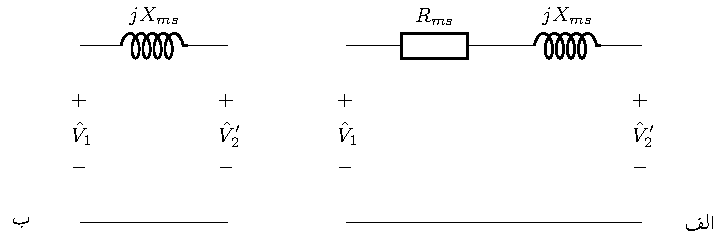
\includegraphics[width=0.9\linewidth]{figTransformersModelCoreLossNeglected}
\caption{ٹرانسفارمر کے سادہ مساوی ادوار۔}
\label{شکل_ٹرانسفارمر_سادہ_ماڈل}
\end{figure}
\حصہ{کھلے دور معائنہ اور کسرِ دور معائنہ}
پچھلے حصے میں بیان کئے گئے ٹرانسفارمر کے مساوی دور کے جزو ٹرانسفارمر کے دو معائنوں سے حاصل کئے جا سکتے ہیں۔ ان معائنوں کو کھلے دور معائنہ اور کسرِ دور معائنہ کہتے ہیں۔اس حصے میں انہیں پر غور کیا جائے گا۔

\جزوحصہ{کھلے دور معائنہ}
کھلے  دور معائنہ\فرہنگ{معائنہ!کھلے دور}\حاشیہب{open circuit test}\فرہنگ{open circuit test} جیسا کہ نام سے واضح  ہے،  ٹرانسفارمر کی ایک جانب لچھے کے سروں کو آزاد رکھ کر کیا جاتا ہے۔ یہ معائنہ اتنی برقی دباو اور تعدد یا ان کے قریب ترین مقداروں پر کیا جاتا ہے جتنے پر ٹرانسفارمر کی بناوٹ\فرہنگ{بناوٹ}\حاشیہب{design} ہو۔ اگرچہ یہ معائنہ ٹرانسفارمر کے کسی بھی جانب کے لچھے پر کیا جا سکتا ہے، حقیقت میں اسے کم برقی دباو والی جانب کے لچھے پر کرنا آسان ہوتا ہے۔یہ بات ایک مثال سے زیادہ آسانی سے سمجھ آتی ہے۔

	مثلاً  ہم  \عددیء{\SI{25}{\kilo \volt \ampere}} اور \عددیء{11000:220\,\textup{V}}  کا \عددیء{\SI{50}{\hertz}} پر چلنے والے ایک دور کے ٹرانسفارمر کا معائنہ کرنا چاہتے ہیں۔ اگر یہ معائنہ اس کے گیارہ ہزار کے لچھے پر  کیا جائے تو گیارہ ہزار برقی دباو کے لگ بھگ برقی دباو استعمال کیا جائے گا اور اگر دو سو بیس برقی دباو والے لچھے پر کیا جائے تو دو سو بیس برقی دباو کے لگ بھگ برقی دباو  استعمال کیا جائے گا۔ دونوں صورتوں میں تعدد \عددیء{\SI{50}{\hertz}} کے لگ بھگ رکھا جائے گی۔\عددیء{\SI{11}{\kilo \volt}} کی برقی دباو پر کام کرنا نہایت خطرناک ثابت ہو سکتا ہے۔یہی وجہ ہے کہ اس معائنہ کو کم برقی دباو والے لچھے پر ہی کیا جاتا ہے۔

 جس برقی دباو پر ٹرانسفارمر عام حالات میں استعمال ہوتا ہے اس معائنہ میں کم برقی دباو والی جانب کے لچھے پر اتنے ہی یا اس کی قریب مقدار کی برقی دباو \عددیء{V_t} لاگو کر کے کھلے دور برقی طاقت \عددیء{p_t} اور  کھلے دور برقی رو \عددیء{I_t}  ناپے جاتے ہیں۔معائنہ حقیقت میں استعمال کے دوران برقی دباو کے جتنے قریب برقی دباو پر کیا جائے اتنا بہتر جواب حاصل ہوتا ہے۔ ٹرانسفارمر کی دوسری جانب لچھے کے سرے چونکہ آزاد رکھے جاتے ہیں اس لئے اس میں  برقی رو صفر ہو گا۔  لہٰذا ناپا گیا برقی رو صرف ہیجان انگیز برقی رو \عددیء{\hat{I}_\varphi} ہو گا۔ ٹرانسفارمر جتنی برقی رو کے لئے بنایا گیا ہو یہ برقی رو اس  کے تقریباً دو سے چھ  فی صد ہوتا ہے۔شکل \حوالہ{شکل_ٹرانسفارمر_مکمل_ماڈل_ابتدائی_جانب}   کو مدِ نظر رکھتے ہوئے اگر ہم بائیں جانب کو کم برقی دباو والی جانب تصور کریں تو شکل میں \عددیء{V_t} کو  \عددیء{V_1} کی جگہ لاگو کرنا ہو گا۔یوں ہم جو برقی رو ناپیں گے وہ  غیر سمتی\حاشیہب{scalar} \عددیء{I_1}  ہو گا۔ چونکہ  \عددیء{I_2'} صفر کے برابر ہے لہٰذا \عددیء{I_1}  درحقیقت \عددیء{\hat{I}_\varphi} کے مقدار \عددیء{I_\varphi} کے برابر ہو گا۔ یعنی  اس  طرح
\begin{align*}
I_t=I_1=I_\varphi
\end{align*}
اتنی کم برقی رو سے لچھے کی رکاوٹ میں نہایت کم برقی دباو گھٹتا ہے،لہٰذا اسے نظر انداز کیا جاتا ہے یعنی
\begin{align*}
V_{R1}&=I_t R_1=I_\varphi R_1 \approx 0\\
V_{X1}&=I_1 X_1=I_\varphi X_1 \approx 0
\end{align*}
یوں  \عددیء{R_c}  اور \عددیء{X_m} پر  تقریباً \عددیء{V_t} برقی دباو پایا جائے گا۔ یہ شکل \حوالہ{شکل_ٹرانسفارمر_مکمل_ماڈل_ابتدائی_جانب}  سے ظاہر ہے۔ان حقائق کو مد نظر رکھتے ہوئے شکل \حوالہ{شکل_ٹرانسفارمر_کھلے_سرے_معائنہ} حاصل ہوتا ہے۔
\begin{figure}
\centering
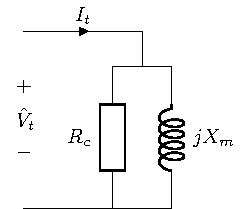
\includegraphics{figTransformersOpenCircuitTest}
\caption{کھلے سرے معائنہ۔}
\label{شکل_ٹرانسفارمر_کھلے_سرے_معائنہ}
\end{figure}

چونکہ برقی طاقت کا ضیاع صرف مزاحمت میں ہی ممکن ہے لہٰذا \عددیء{p_t} صرف  \عددیء{R_c}  میں ہی ضائع ہو گی۔ یوں
\begin{align*}
p_t=\frac{V_t^2}{R_c}
\end{align*}
لکھا جائے گا۔یوں
\begin{align}\label{مساوات_ٹرانسفارمر_کھلے_دور_مزاحمت_حاصل}
R_c&=\frac{V_t^2}{p_t}
\end{align}
حاصل ہوتا ہے۔

اسی طرح چونکہ برقی دباو اور برقی رو کی مقداروں کے تناسب کو برقی رکاوٹ کی مقدار کہتے ہیں لہٰذا
\begin{align*}
\abs{Z_t}=\frac{V_t}{I_t}
\end{align*}
مگر شکل \حوالہ{شکل_ٹرانسفارمر_کھلے_سرے_معائنہ}  سے واضح ہے کہ
\begin{align*}
\frac{1}{Z_t}=\frac{1}{R_c}+\frac{1}{j X_m}
\end{align*}
لہٰذا
\begin{align*}
Z_t&=\frac{j R_c X_m}{R_c+j X_m}\\
\abs{Z_t}&=\frac{R_c X_m}{\sqrt{R_c^2+X_m^2}}
\end{align*}
جس سے حاصل ہوتا ہے
\begin{align}\label{مساوات_ٹرانسفارمر_کھلے_دور_امالہ_حاصل}
X_m=\frac{R_c \abs{Z_t}}{\sqrt{R_c^2-\abs{Z_t}^2}}
\end{align}
مساوات \حوالہ{مساوات_ٹرانسفارمر_کھلے_دور_مزاحمت_حاصل}  سے \عددیء{R_c} اور  مساوات \حوالہ{مساوات_ٹرانسفارمر_کھلے_دور_امالہ_حاصل}  سے  \عددیء{X_m}  کا حساب لگایا جاتا ہے۔

یاد رہے کہ حاصل کردہ \عددیء{R_c} اور \عددیء{X_m} ٹرانسفارمر کے اسی جانب کے لئے درست ہیں جس جانب انہیں حاصل کیا گیا ہو۔اگر ان کی قیمتیں دوسری جانب درکار ہوں تب تبادلہ رکاوٹ کا استعمال کرتے ہوئے اس جانب کی قیمتیں حاصل کی جا سکتی ہیں۔ 

\جزوحصہ{ کسرِ دور معائنہ}
یہ معائنہ بھی پچھلے معائنہ کی طرح ٹرانسفارمر کے کسی بھی طرف کیا جا سکتا ہے مگر حقیقت میں اسے زیادہ برقی دباو کے لچھے پر ہی کرنا زیادہ آسان ہوتا ہے۔ یہ معائنہ جتنے برقی رو کے لئے ٹرانسفارمر بنایا گیا ہو اتنی برقی رو یا اس کے قریب مقدار پر کیا جاتا ہے۔یعنی اس معائنہ میں کوشش ہوتی ہے کہ ٹرانسفارمر کے لچھے میں اتنی برقی رو گزرے جتنی کے لئے یہ بنایا گیا ہو۔ لہٰذا اگر ہم پچھلے معائنہ میں استعمال ہونے والے ٹرانسفارمر کی بات آگے بڑھائیں تو اس کا زیادہ برقی دباو کا لچھا \عددیء{\SI{2.2727}{\ampere}} اور کم برقی دباو کا لچھا \عددیء{\SI{113.63}{\ampere}} کے لئے بنایا گیا ہے۔ لہٰذا اگر یہ معائنہ کم برقی دباو لچھے پر کیا جائے تو اسے \عددیء{\SI{113.63}{\ampere}}  پر  کرنا ہو گا اور اگر زیادہ برقی دباو لچھے پر کیا جائے تو صرف \عددیء{\SI{2.2727}{\ampere}} پر کرنا ہو گا جو کہ زیادہ آسان ہے۔
\begin{figure}
\centering
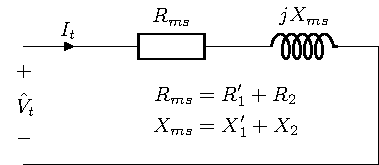
\includegraphics{figTransformersShortCircuitTest}
\caption{کسر دور معائنہ۔}
\label{شکل_ٹرانسفارمر_کسر_دور_معائنہ}
\end{figure}

اس معائنہ میں کم برقی دباو لچھے کے دونوں سروں کو آپس میں جوڑا جاتا ہے یعنی انہیں کسرِ دور کر لیا جاتا ہے اور زیادہ برقی دباو لچھے پر اس جانب کی ڈیزائن کردہ برقی دباو کے دو سے بارہ  فی صد کا برقی دباو \عددیء{V_t} لاگو کر کے کسرِ دور برقی رو \عددیء{I_t} اور کسرِ دور برقی طاقت \عددیء{p_t} ناپے جاتے ہیں۔ جس لچھے کے سرے آپس میں کسرِ دور ہوتے ہیں اس میں سے برقی رو گزرتی ہے اور اس کا عکس دوسری جانب بھی موجود ہوتا ہے۔ یہ برقی رو ٹرانسفارمر کے ڈیزائن کردہ برقی رو کے لگ بھگ ہوتا ہے۔ اس معائنہ کا دور شکل \حوالہ{شکل_ٹرانسفارمر_کسر_دور_معائنہ} میں دکھایا گیا ہے۔کھلے سرے معائنے کی طرح اگر کسر دور معائنے میں بھی  شکل \حوالہ{شکل_ٹرانسفارمر_مکمل_ماڈل_ابتدائی_جانب} کے بائیں جانب کو کم برقی دباو والی جانب تصور کریں تو  \عددیء{V_t} کو  \عددیء{V_2} کی جگہ لاگو کرنا ہو گا۔

 چونکہ یہ معائنہ بہت کم برقی دباو پر کیا جاتا ہے لہٰذا اس معائنہ میں ہیجان انگیز برقی رو کو مکمل طور پر نظرانداز کیا جا سکتا ہے۔ شکل سے ہم دیکھتے ہیں کہ چونکہ برقی طاقت صرف مزاحمت میں ہی ضائع ہو سکتی ہے لہٰذا
\begin{align*}
p_t=I_t^2 \left(R_{ms}\right)
\end{align*}
ہو گا جس سے
\begin{align}\label{مساوات_ٹرانسفارمر_کسر_دور_مزاحمت_حاصل}
R_{ms}=\frac{p_t}{I_t^2}
\end{align}
حاصل ہوتا ہے۔

کسرِ دور برقی رو اور برقی دباو سے ہمیں ملتی ہے
\begin{align*}
\abs{Z_t}=\frac{V_t}{I_t}
\end{align*}
مگر شکل سے واضح ہے کہ
\begin{align*}
Z_t&=R_{ms}+j X_{ms}\\
\abs{Z_t}&=\sqrt{R_{ms}^2+X_{ms}^2}
\end{align*}
لہٰذا
\begin{align}\label{مساوات_ٹرانسفارمر_کسر_دور_امالہ_حاصل}
X_{ms}=\sqrt{\abs{Z_t}^2-R_{ms}^2}
\end{align}
مساوات \حوالہ{مساوات_ٹرانسفارمر_کسر_دور_مزاحمت_حاصل} کُل مزاحمت دیتا ہے البتہ اس سے \عددی{R_1} یا \عددیء{R_2} حاصل نہیں کیا جا سکتا۔اسی طرح مساوات \حوالہ{مساوات_ٹرانسفارمر_کسر_دور_امالہ_حاصل} سے \عددیء{X_1} اور \عددیء{X_2} علیحدہ نہیں کئے جا سکتے۔کسر دور معائنہ سے اتنی ہی معلومات حاصل کرنا ممکن ہے۔حقیقت میں اتنی معلومات کافی ہوتی ہے۔ اگر ان اجزاء ک علیحدہ علیحدہ قیمتیں درکار ہوں تو ایسی صورت میں تصور کیا جاتا ہے کہ
\begin{align*}
R_1'&=R_2\\
X_1'&=X_2
\end{align*}
ہیں۔

 چونکہ یہ معائنہ عموماً جہاں ٹرانسفارمر موجود ہو وہیں کرنا پڑتا ہے لہٰذا یہ ممکن نہیں ہوتا کہ ٹرانسفارمر کو بالکل اتنا برقی دباو دیا جائے جتنا درکار ہو بلکہ جو برقی دباو موجود ہو اسی سے کام چلانا پڑتا ہے۔ لیکن اس بات کا خیال بہت ضروری ہے کہ جو برقی دباو ٹرانسفارمر کو دیا جا رہا ہو وہ ڈیزائن کردہ برقی دباو کے دو سے بارہ  فی صد ہو۔ مثلاً اگر اسی \عددیء{11000:220\,\textup{V}} ٹرانسفارمر کی بات کی جائے تو اس کے زیادہ برقی دباو لچھے پر \عددیء{\SI{220}{\volt}} اور \عددیء{\SI{1320}{\volt}}  کے درمیان کوئی بھی برقی دباو دیا جا سکتا ہے۔ چونکہ ہمارے ہاں \عددیء{\SI{220}{\volt}}  اور \عددیء{\SI{440}{\volt}}  عام پائے جاتے ہیں لہٰذا ہم \عددیء{\SI{220}{\volt}}  یا \عددیء{\SI{440}{\volt}}  ہی استعمال کریں گے۔

یہاں یہ ایک مرتبہ دوبارہ یاد دھیانی کراتا جاول کہ ٹرانسفارمر کی ایک جانب لچھے کے سرے آپس میں جوڑ کر، یعنی انہیں کسرِ دور کر کے، دوسری جانب لچھے پر کسی بھی صورت میں اس جانب کی پوری برقی دباو لاگو نہیں کرنا۔ ایسا کرنا  شدید  خطرناک اور جان لیوا ثابت ہو سکتا ہے۔

یاد رہے کہ حاصل کردہ \عددیء{R_c} اور \عددیء{X_m} ٹرانسفارمر کے اسی جانب کے لئے درست ہیں جس جانب انہیں حاصل کیا گیا ہو۔اگر ان کی قیمتیں دوسری جانب درکار ہوں تب تبادلہ رکاوٹ کا استعمال کرتے ہوئے اس جانب کی قیمتیں حاصل کی جا سکتی ہیں۔ 
%
\ابتدا{مثال}
ایک \عددیء{25}  کلو وولٹ-ایمپیئر، \عددیء{11000:220} وولٹ اور \عددیء{50} ہرٹز پر چلنے والے ٹرانسفارمر کے کھلے دور اور کسرِ دور معائنہ کئے جاتے ہیں جن کے نتائج یہ ہیں۔
\begin{itemize}
\item
کھلے دور معائنہ کرتے وقت کم برقی دباو کی جانب  \عددیء{\SI{220}{\volt}} لاگو کئے جاتے ہیں۔اسی جانب برقی رو \عددیء{\SI{39.64}{\ampere}} اور طاقت کا ضیاع \عددیء{\SI{600}{\watt}} ناپے جاتے ہیں۔
\item
کسرِ دور معائنہ کرتے وقت زیادہ برقی دباو کی جانب  \عددیء{\SI{440}{\volt}} لاگو کئے جاتے ہیں۔اسی جانب برقی رو \عددیء{\SI{2.27}{\ampere}} اور طاقت کا ضیاع \عددیء{\SI{560}{\watt}} ناپے جاتے ہیں۔
\end{itemize}

کھلے دور حل:
\begin{align*}
\abs{Z_t}&=\frac{220}{39.64}=\SI{5.55}{\ohm}\\
R_c&=\frac{220^2}{600}=\SI{80.67}{\ohm}\\
X_m&=\frac{80.67 \times 5.55}{\sqrt{80.67^2-5.55^2}}=\SI{5.56}{\ohm}
\end{align*}
کسر دور حل:
\begin{align*}
Z_t&=\frac{440}{2.27}=\SI{193.83}{\ohm}\\
R_{ms}&=\frac{560}{2 \times 2.27^2}=\SI{108.68}{\ohm}\\
X_{ms}&=\sqrt{193.83^2-108.68^2}=\SI{160}{\ohm}
\end{align*}

ان نتائج کو کم برقی دباو جانب منتقل کرتے ہوئے 
\begin{align*}
\left(\frac{220}{11000} \right)^2 \times 108.68=\SI{43.47}{\milli \ohm}\\
\left(\frac{220}{11000} \right)^2 \times 160=\SI{64}{\milli \ohm}
\end{align*}
یعنی
\begin{align*}
R_1&=R_2'=\frac{\SI{43.47}{\milli \ohm}}{2}=\SI{21.7}{\milli \ohm}\\
X_1&=X_2'=\frac{\SI{64}{\milli \ohm}}{2}=\SI{32}{\milli \ohm}
\end{align*}
حاصل ہوتا ہے۔ان نتائج سے حاصل کم برقی دباو جانب مساوی دور شکل \حوالہ{شکل_ٹرانسفارمر_کھلے_سرے_کسر_دور_مثال} میں دکھایا گیا ہے۔
\begin{figure}
\centering
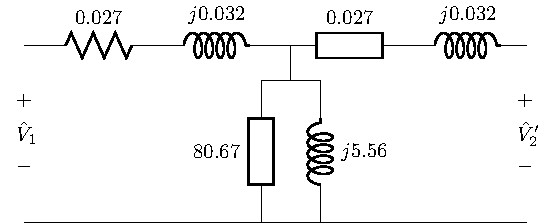
\includegraphics{figTransformersOpenAndShortTestExample}
\caption{کھلے دور اور کسرِ دور معائنہ سے کم برقی دباو جانب  مساوی دور۔}
\label{شکل_ٹرانسفارمر_کھلے_سرے_کسر_دور_مثال}
\end{figure}
\انتہا{مثال}
%
\حصہ{تین مرحلہ ٹرانسفارمر}
اب تک ہم  \اصطلاح{ایک مرحلہ}\حاشیہب{single phase} ٹرانسفارمر پر غور کرتے رہے ہیں۔حقیقت میں برقی طاقت کی منتقلی میں عموماً \اصطلاح{تین مرحلہ}\فرہنگ{تین مرحلہ}\حاشیہب{three phase}\فرہنگ{three phase} ٹرانسفارمر استعمال ہوتے ہیں۔تین مرحلہ ٹرانسفارمر یکساں تین عدد  ایک مرحلہ  ٹرانسفارمر اکٹھے رکھ کر بنایا جا سکتا ہے۔یوں اگر ایک ٹرانسفارمر خراب ہو جائے تو اس کو ٹھیک ہونے کے لئے ہٹا کر بقایا دو ٹرانسفارمر دوبارہ چالو کئے جا سکتے ہیں۔تین مرحلہ ٹرانسفارمر بنانے کا اس سے بہتر طریقہ شکل \حوالہ{شکل_ٹرانسفارمر_ایک_مرکز_تین-ٹرانسفارمر} میں دکھایا گیا ہے جہاں ایک ہی مقناطیسی قالب پر تینوں ٹرانسفارمر کے لچھے لپٹے گئے ہیں۔اس شکل میں \عددیء{\hat{V}_{i1}} پہلے ٹرانسفارمر کا ابتدائی لچھا جبکہ \عددیء{\hat{V}_{s1}} اس کا ثانوی لچھا ہے۔اس طرح کے تین مرحلہ ٹرانسفارمر سستے، ہلکے اور چھوٹے ہونے کی وجہ سے عام ہو گئے ہیں اور آپ کو روز مرہ زندگی میں یہی نظر آئیں گے۔ان میں برقی ضیاع بھی قدرِ کم ہوتی ہے۔
\begin{figure}
\centering
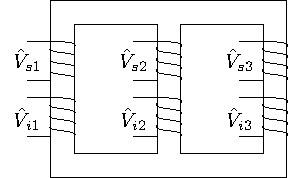
\includegraphics{figTransformersThreePhaseSingleCore}
\caption{ایک ہی قالب پر تین ٹرانسفارمر۔}
\label{شکل_ٹرانسفارمر_ایک_مرکز_تین-ٹرانسفارمر}
\end{figure}

شکل \حوالہ{شکل_ٹرانسفارمر_ستارہ_تکونی_جوڑ}-الف میں تین ٹرانسفارمر دکھائے گئے ہیں۔ان تین ٹرانسفارمر کے ابتدائی لچھے آپس میں دو طریقوں سے جوڑے جا سکتے ہیں۔ایک کو \اصطلاح{ستارہ نما} جوڑ\فرہنگ{ستارہ نما جوڑ}\فرہنگ{جوڑ!ستارہ نما}\حاشیہب{star connected}\فرہنگ{star connected} \عددیء{Y}  اور دوسرے کو \اصطلاح{تکونی} جوڑ\فرہنگ{تکونی جوڑ}\فرہنگ{جوڑ!تکونی}\حاشیہب{delta connected}\فرہنگ{delta connected}  \عددیء{\Delta}   کہتے ہیں۔اسی طرح ان تینوں ٹرانسفارمروں کے ثانوی  لچھے انہیں دو طریقوں سے جوڑے جا سکتے ہیں۔یوں انہیں جوڑنے کے چار ممکنہ طریقے ہیں یعنی
\begin{itemize}
\item
ستارہ:تکونی  \quad \عددیء{Y:\Delta}
\item
ستارہ:ستارہ \quad  \عددیء{Y:Y}
\item
تکونی:تکونی \quad  \عددیء{\Delta:\Delta}
\item
تکونی:ستارہ  \quad  \عددیء{\Delta:Y}
\end{itemize}

شکل \حوالہ{شکل_ٹرانسفارمر_ستارہ_تکونی_جوڑ}-الف میں ان تین ٹرانسفارمروں کے ابتدائی لچھوں کو ستارہ نما جوڑا گیا ہے جبکہ ان کی ثانوی لچھوں کو تکونی جوڑا گیا ہے۔شکل-ب میں تینوں ٹرانسفارمر کی ابتدائی لچھوں کو  ستارہ نما  دکھایا گیا ہے۔اسی طرح ثانوی لچھوں کو تکونی  دکھایا گیا ہے۔انہی شکلوں کی وجہ سے ان کو ستارہ نما جوڑ اور تکونی جوڑ کہتے ہیں۔

ایسی شکل بناتے وقت تینوں ٹرانسفارمروں کے ابتدائی لچھے کو جس زاویہ پر بنایا جاتا ہے اس کے ثانوی لچھے کو بھی اُسی زاویہ پر بنایا جاتا ہے۔یوں شکل کے حصہ الف میں سب سے اوپر ٹرانسفارمر جس کے ابتدائی جانب کے  سرے \عددیء{an} اور ثانوی جانب  کے سرے \عددیء{a'n'} ہیں کو حصہ با میں صفر زاویہ پر بنایا گیا ہے۔تین  مرحلہ ٹرانسفارمروں کو اس طرح کی علامتوں سے ظاہر کیا جاتا ہے اور ان میں قالب نہیں دکھایا جاتا۔

ٹرانسفارمر کے جوڑ بیان کرتے وقت بائیں جانب کے جوڑ کو پہلے اور دائیں جانب کی جوڑ کو بعد میں پکارتے ہیں۔یوں شکل میں ٹرانسفارمر کو ستارہ-تکونی جُڑا ٹرانسفارمر کہیں گے۔اسی طرح ابتدائی جانب کو بائیں اور ثانوی جانب کو دائیں ہاتھ بنایا جاتا ہے۔یوں اس شکل میں ابتدائی جانب ستارہ نما ہے جبکہ ثانوی جانب تکونی ہے۔
\begin{figure}
\centering
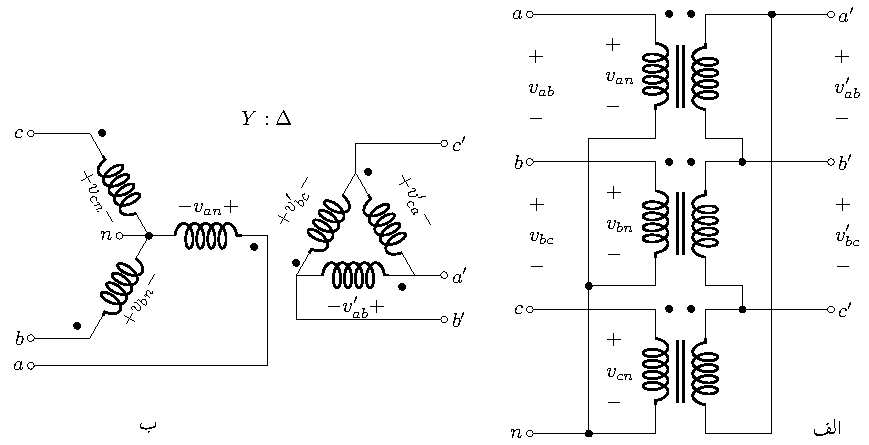
\includegraphics[width=\linewidth]{figTransformersStarDeltaConnections}
\caption{تین مرحلہ ستارہ-تکونی ٹرانسفارمر}
\label{شکل_ٹرانسفارمر_ستارہ_تکونی_جوڑ}
\end{figure}


	ستارہ نما جڑی جانب سے چار برقی تاریں نکلتی ہیں۔اس جانب لچھوں کے مشترکہ سرا \عددیء{n} کو عموماً ٹرانسفارمر کے نزدیک زمین میں گہرائی تک دھنسا دیا جاتا ہے۔اس تار کو \اصطلاح{زمینی تار}\فرہنگ{زمینی تار}\حاشیہب{ground}\فرہنگ{ground wire}  یا صرف \اصطلاح{زمین}\فرہنگ{زمین}\حاشیہب{ground, earth,neutral}\فرہنگ{earth}  کہتے ہیں۔عام فہم میں اسے \اصطلاح{ٹھنڈی تار}\فرہنگ{ٹھنڈی تار}\حاشیہب{neutral} کہتے ہیں۔باقی تین یعنی \عددیء{a,b,c}  \اصطلاح{گرم تار}\فرہنگ{گرم تار}\حاشیہب{live wires} کہلاتے ہیں۔

ٹرانسفارمر کی لچھے پر برقی دباو کو \اصطلاح{یک مرحلہ برقی دباو}\فرہنگ{یک مرحلہ برقی دباو} \عددیء{\hat{V}_{\textup{یکمرحلہ}}}\حاشیہب{phase voltage}\فرہنگ{phase voltage} کہتے ہیں اور لچھے میں برقی رو کو \اصطلاح{یک مرحلہ برقی رو}\فرہنگ{یک مرحلہ برقی رو} \عددیء{\hat{I}_{\textup{یکمرحلہ}}}\حاشیہب{phase current}\فرہنگ{phase current}  کہتے ہیں۔ جبکہ ٹرانسفارمر سے باہر نکلتی کسی دو گرم تاروں کے مابین برقی دباو کو \اصطلاح{تار کی برقی دباو}\فرہنگ{تار کی برقی دباو} \عددیء{\hat{V}_{\textup{تار}}}\حاشیہب{line to line voltage}\فرہنگ{line voltage} کہتے ہیں اور کسی بھی گرم تار میں برقی رو کو \اصطلاح{تار کی برقی رو}\فرہنگ{تار کی برقی رو} \عددیء{\hat{I}_{\textup{تار}}}\حاشیہب{line current}\فرہنگ{line current}  کہتے ہیں۔ زمینی تار میں برقی رو کو \اصطلاح{زمینی برقی رو}\فرہنگ{زمینی برقی رو}  \عددیء{\hat{I}_{\textup{زمینی}}}\حاشیہب{ground current}\فرہنگ{ground current} کہتے ہیں۔

ستارہ نما \عددیء{Y} جانب \اصطلاح{یک مرحلہ} مقداروں اور \اصطلاح{تار} کی مقداروں  کا آپس میں یوں رشتہ ہے
\begin{gather}
\begin{aligned}\label{مساوات_ستارہ_ٹرانسفارمر_تار_اور_دور_رشتے}
V_{\textup{تار}}&=\sqrt{3} V_{\textup{یکمرحلہ}}\\
I_{\textup{تار}}&=I_{\textup{یکمرحلہ}}
\end{aligned}
\end{gather}
جبکہ تکونی \عددیء{\Delta} جانب یک مرحلہ اور تار کی مقداروں کا آپس میں یوں رشتہ ہے
\begin{gather}
\begin{aligned}\label{مساوات_تکونی_ٹرانسفارمر_تار_اور_دور_رشتے}
V_{\textup{تار}}&= V_{\textup{یکمرحلہ}}\\
I_{\textup{تار}}&=\sqrt{3} I_{\textup{یکمرحلہ}}
\end{aligned}
\end{gather}
یہ مرحلی سمتیہ کے رشتے نہیں بلکہ ان کی غیر سمتی قیمتوں کے رشتے ہیں۔ان دو مساواتوں سے حاصل ہوتا ہے
\begin{align}
V_{\textup{تار}} I_{\textup{تار}}=\sqrt{3} V_{\textup{یکمرحلہ}} I_{\textup{یکمرحلہ}}
\end{align}
چونکہ ایک مرحلہ ٹرانسفارمر کی وولٹ-ایمپیئر \عددیء{V_{\textup{یکمرحلہ}} I_{\textup{یکمرحلہ}}} ہیں اور ایسے تین ٹرانسفارمر مل کر ایک تین مرحلہ ٹرانسفارمر بناتے ہیں لہٰذا تین  مرحلہ ٹرانسفارمر کی وولٹ-ایمپیئر اس کے تین گنا ہوں گے یعنی
\begin{align}
\textup{وولٹ-ایمپیئر}= 
3 V_{\textup{یکمرحلہ}} I_{\textup{یکمرحلہ}}= 
3 \times \frac{V_{\textup{تار}} I_{\textup{تار}}}{\sqrt{3}}=
\sqrt{3} V_{\textup{تار}} I_{\textup{تار}}
\end{align}
یہ مساوات \اصطلاح{تین مرحلہ} ادوار  میں عام استعمال ہوتی ہے۔

	ٹرانسفارمر کسی طرح بھی جوڑے جائیں وہ اپنی بنیادی کارکردگی تبدیل نہیں کرتے لہٰذا انہیں ستارہ نما یا تکونی جوڑنے کے بعد بھی ان میں ہر ایک ٹرانسفارمر انفرادی طور پر صفحہ \حوالہصفحہ{مساوات_ٹرانسفارمر_تبادلہ_دباو_رو} پر دئے مساوات \حوالہ{مساوات_ٹرانسفارمر_تبادلہ_دباو_رو}  اور صفحہ \حوالہصفحہ{مساوات_ٹرانسفارمر_متبادل_رکاوٹ_تعریف} پر دئے مساوات \حوالہ{مساوات_ٹرانسفارمر_متبادل_رکاوٹ_تعریف}  پر پورے اترے گا۔انہیں استعمال کر کے شکل \حوالہ{شکل_ٹرانسفارمر_تین_دور_ٹرانسفارمر_کے_مختلف_جوڑ}  میں دیئے گئے ٹرانسفارمروں کے ابتدائی اور ثانوی جانب کی یک مرحلہ اور تار کی مقداروں کے رشتے حاصل کئے جا سکتے ہیں۔اس شکل میں \عددیء{a=N_1/N_2} ہے جہاں  \عددیء{N_1:N_2} ان میں ایک مرحلہ ٹرانسفارمر کے چکر کی نسبت ہے۔تین مرحلہ ٹرانسفارمر پر لگی تختی پر دونوں جانب تار کی برقی دباو کی نسبت لکھی جاتی ہے۔
\begin{figure}
\centering
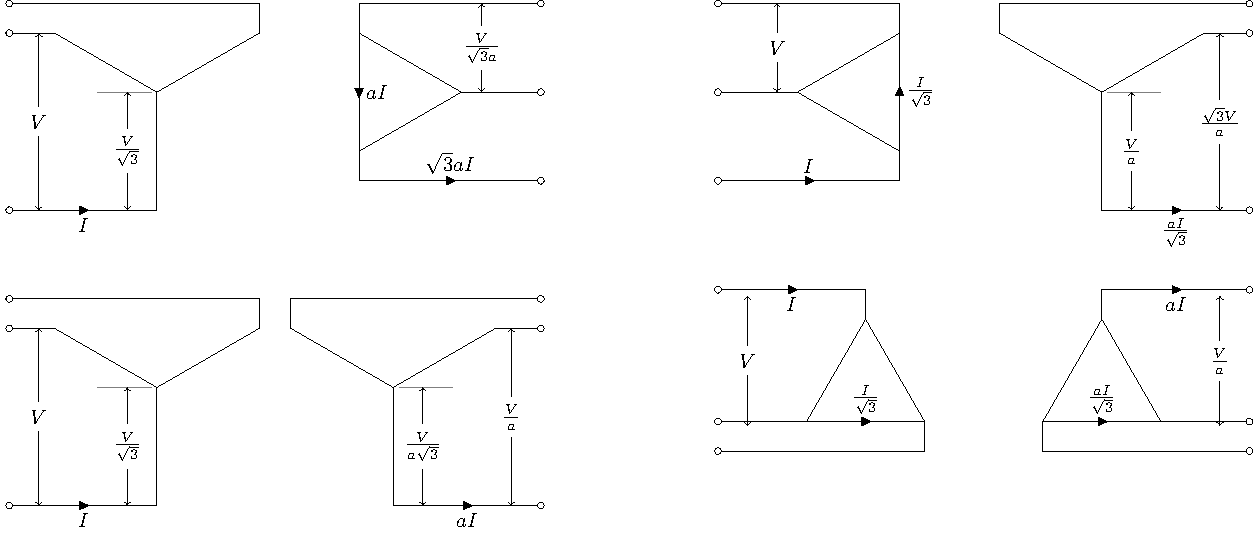
\includegraphics[width=\linewidth]{figTransformersAllPossibleConnections}
\caption{ابتدائی اور ثانوی جانب تار اور یک مرحلہ مقداروں کے رشتے۔}
\label{شکل_ٹرانسفارمر_تین_دور_ٹرانسفارمر_کے_مختلف_جوڑ}
\end{figure}


جیسے شکل \حوالہ{شکل_ٹرانسفارمر_تین_دور_ٹرانسفارمر_کے_مختلف_جوڑ} میں دکھایا گیا ہے ستارہ-تکونی ٹرانسفارمر کی تار پر برقی دباو کی نسبت
\begin{align}
\frac{V_\textup{{ابتدائی}}}{V_\textup{{ثانوی}}}=\sqrt{3} a =\sqrt{3} \left(\frac{N_1}{N_2} \right)
\end{align}
جبکہ ستارہ-ستارہ کا
\begin{align}
\frac{V_\textup{{ابتدائی}}}{V_\textup{{ثانوی}}}=a =\left(\frac{N_1}{N_2} \right)
\end{align}
تکونی-ستارہ کا
\begin{align}
\frac{V_\textup{{ابتدائی}}}{V_\textup{{ثانوی}}}=\frac{a}{\sqrt{3}}=\frac{1}{\sqrt{3}} \left(\frac{N_1}{N_2} \right)
\end{align}
اور تکونی-تکونی کا
\begin{align}
\frac{V_\textup{{ابتدائی}}}{V_\textup{{ثانوی}}}=a =\left(\frac{N_1}{N_2} \right)
\end{align}
ہے۔
%
\ابتدا{مثال}
یک مرحلہ  تین یکساں ٹرانسفارمروں کو ستارہ-تکونی \عددیء{Y:\Delta}  جوڑ کر تین مرحلہ ٹرانسفارمر بنایا گیا ہے۔ایک مرحلہ ٹرانسفارمر کی برقی \اصطلاح{سکت}\فرہنگ{سکت}\حاشیہب{rating}\فرہنگ{rating} درج ذیل ہے:
\begin{align*}
\SI{50}{\kilo \volt \ampere} , \quad 6350:440\,\textup{V}, \quad \SI{50}{\hertz}
\end{align*}
ستارہ-تکونی ٹرانسفارمر کی ابتدائی جانب \عددیء{11000}  وولٹ کی تین مرحلہ تار کی برقی دباو لاگو کیا گیا۔اس تین مرحلہ ٹرانسفارمر کی ثانوی جانب تار کا برقی دباو معلوم کریں۔

حل: حل کرتے وقت ہم ایک  عدد  یک مرحلہ ٹرانسفارمر پر نظر رکھیں گے۔ ابتدائی جانب اگر یک مرحلہ ٹرانسفارمر پر غور کیا جائے تو
\begin{align*}
\frac{N_1}{N_2}=\frac{V_1}{V_2}=\frac{6350}{440}
\end{align*}
اور اس پر لاگو برقی دباو مساوات \حوالہ{مساوات_ستارہ_ٹرانسفارمر_تار_اور_دور_رشتے}  کی مدد سے
\begin{align*}
V_{\textup{ابتدائی، یکمرحلہ}}=\frac{V_{\textup{تار}}}{\sqrt{3}}=\frac{11000}{\sqrt{3}}=\SI{6350.85}{\volt}
\end{align*}
ہے لہٰذا اس یک مرحلہ ٹرانسفارمر کی ثانوی جانب مساوات \حوالہ{مساوات_ٹرانسفارمر_تبادلہ_دباو_رو} کی مدد سے
\begin{align*}
V_{\textup{ثانوی}}=\frac{N_2}{N_1} V_{\textup{ابتدائی}}=\frac{440}{6350} \times 6350.85 \approx \SI{440}{\volt}
\end{align*}
ہیں۔چونکہ ثانوی جانب ان تین یک مرحلہ ٹرانسفارمروں کو تکونی جوڑا گیا ہے لہٰذا مساوات \حوالہ{مساوات_تکونی_ٹرانسفارمر_تار_اور_دور_رشتے}  کی مدد سے اس جانب تار کی برقی دباو یہی ہو گی۔اس تین مرحلہ ٹرانسفارمر کی تار پر برقی دباو کی نسبت
\begin{align*}
\frac{V_{\textup{ابتدائی، تار}}}{V_{\textup{ثانوی، تار}}}=\frac{11000}{440}
\end{align*}
ہے۔چونکہ یک مرحلہ ٹرانسفارمر \عددیء{50}  کلو وولٹ-ایمپیئر کا ہے لہٰذا یہ تین مرحلہ ٹرانسفارمر  \عددیء{150} کلو وولٹ-ایمپیئر کا ہو گا۔یوں اس تین مرحلہ ٹرانسفارمر کی سکت\فرہنگ{سکت}\حاشیہب{rating}\فرہنگ{rating}
\begin{align*}
\SI{150}{\kilo \volt \ampere}, \quad 11000:440\,\textup{V},\quad \SI{50}{\hertz}
\end{align*}
ہو گی۔

	ٹرانسفارمر پر لگی تختی\فرہنگ{تختی}\حاشیہب{name plate}\فرہنگ{name plate} پر اس کی سکت بیان ہوتی ہے جس میں ٹرانسفارمر کے دونوں جانب تار کے برقی دباو لکھے جاتے ہیں نہ کہ لچھوں کے چکر۔
\انتہا{مثال}
%
ستارہ-ستارہ جڑے ٹرانسفارمر عام طور استعمال نہیں ہوتے۔اس کی وجہ یہ ہے کہ اگرچہ ان کی تین مرحلہ برقی دباو  کے بنیادی جزو آپس میں \عددیء{120\degree}  زاویائی فاصلے پر ہوتے ہیں لیکن ان کی تیسری موسیقائی جزو آپس میں ہم قدم ہوتی ہیں۔قالب کی غیر بتدریج خصوصیات کی وجہ سے ٹرانسفارمر میں ہر صورت تیسری موسیقائی جزو پائے جاتے ہیں۔تیسری موسیقائی جزو ہم قدم ہونے کی وجہ سے جمع ہو کر ایک نہایت بڑی برقی دباو کی موج پیدا کرتے ہیں جو کبھی کبھی برقی دباو کی بنیادی جزو سے بھی زیادہ بڑھ جاتی ہے۔

بقایا تین قسم کے جڑے ٹرانسفارمروں میں برقی دباو کی تیسری موسیقائی جزو مسئلہ نہیں کرتیں چونکہ ان میں تکونی جُڑے لچھوں میں برقی رو گھومنے شروع ہو جاتی ہے جو ان کے اثر کو ختم کر دیتی ہے۔

تین مرحلہ ٹرانسفارمر کے متوازن دور حل کرتے وقت ہم تصور کرتے ہیں کہ ٹرانسفارمر ستارہ نما جڑا  ہے۔یوں اس کے ایک مرحلے میں برقی رو، تار  کی برقی رو ہی ہو گی اور اس کے ایک مرحلے پر لاگو برقی دباو، یک مرحلہ برقی دباو  ہو گا۔اسی طرح ہم تصور کرتے ہیں کہ اس پر لدا برقی بوجھ بھی ستارہ نما جُڑا ہے۔یوں تین مرحلہ کی جگہ ہم یک مرحلہ دور کا نسبتاً آسان مسئلہ حل کرتے ہیں۔ ایسا کرنے سے مسئلہ پر غور کرنا آسان ہو جاتا ہے۔یہ ایک مثال سے زیادہ بہتر سمجھ آئے گا۔
%
\ابتدا{مثال}
ایک تین مرحلہ \عددیء{\Delta :Y}   \عددیء{2000} کلو وولٹ-ایمپیئر،  \عددیء{11000:600 }  وولٹ اور \عددیء{50} ہرٹز پر چلنے والا کامل ٹرانسفارمر تین مرحلہ کے متوازن برقی بوجھ کو طاقت مہیا کر رہا ہے۔یہ بوجھ تکونی جڑا ہے جہاں بوجھ کا ہر حصہ \عددیء{(0.504+j0.1917)} کے برابر ہے۔شکل \حوالہ{شکل_ٹرانسفارمر_تکونی_بار_کی_مثال}  میں یہ دکھایا گیا ہے۔
\begin{itemize}
\item
اس شکل میں ہر جگہ برقی رو معلوم کریں۔
\item
برقی بوجھ\فرہنگ{بوجھ}\حاشیہب{electrical load}\فرہنگ{load} کو درکار طاقت معلوم کریں
\end{itemize}

\begin{figure}
\centering
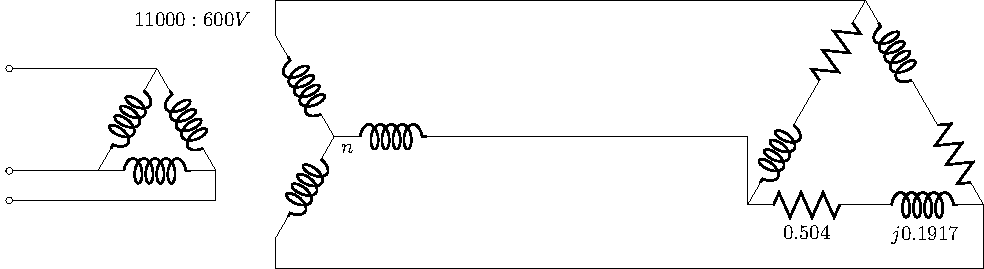
\includegraphics[width=\linewidth]{figTransformersDeltaLoadedExample}
\caption{ٹرانسفارمر تکونی متوازن بوجھ کو طاقت فراہم کر رہا ہے۔}
\label{شکل_ٹرانسفارمر_تکونی_بار_کی_مثال}
\end{figure}
حل:

پہلے تکونی بوجھ کو ستارہ نما بوجھ میں تبدیل کرتے ہیں
\begin{align*}
Z_Y= \frac{Z_\Delta}{3}=\frac{0.504+j0.1917}{3}=0.168+j0.0639
\end{align*}
اس بوجھ کو ستارہ نما جڑا شکل \حوالہ{شکل_ٹرانسفارمر_تکونی_بار_کو_ستارہ_تبادلہ} میں دکھایا گیا ہے۔اس شکل میں ایک برقی تار جسے نقطہ دار لکیر سے ظاہر کیا گیا ہے کو ٹرانسفارمر کی زمینی نقطہ سے بوجھ کے مشترکہ سرے کے درمیان جڑا دکھایا گیا ہے۔متوازن دور میں اس تار میں برقی رو صفر ہو گی۔حل کرنے کی نیت سے ہم اس متوازن دور سے ایک مرحلہ لے کر حل کرتے ہیں۔
\begin{figure}
\centering
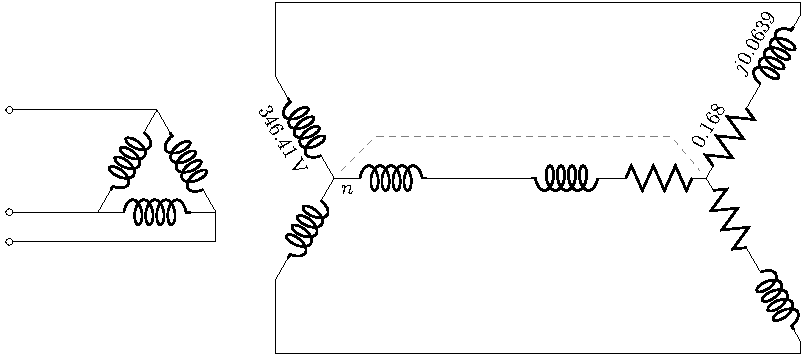
\includegraphics[width=\linewidth]{figTransformersDeltaLoadedExampleTurnedStar}
\caption{تکونی بوجھ کو مساوی ستارہ بوجھ میں تبدیل کیا گیا ہے۔}
\label{شکل_ٹرانسفارمر_تکونی_بار_کو_ستارہ_تبادلہ}
\end{figure}

یوں مساوی برقی بوجھ میں برقی رو
\begin{align*}
I=\frac{346.41}{0.168+j0.0639}=1927.262\phase{-20.825\degree}
\end{align*}
ہو گی اور اس ایک مرحلہ میں طاقت
\begin{align*}
p=346.41 \times 1927.262 \times \cos (-20.825\degree)=\SI{624007}{\watt}
\end{align*}
ہو گی۔ یوں برقی بوجھ کو پوری درکار برقی طاقت اس کے تین گنا ہو گی یعنی \عددیء{\SI{1872}{\kilo \watt}}  اس بوجھ کا جزو طاقت\حاشیہب{power factor} 
\begin{align*}
\cos (-20.825\degree)=0.93467
\end{align*}
ہے۔

	تکونی بوجھ   میں برقی رو \عددیء{\tfrac{1927.262}{\sqrt{3}}=1112.7} ایمپیئر ہو گی۔ ٹرانسفارمر کی ابتدائی جانب برقی تاروں میں برقی رو
\begin{align*}
\left(\frac{600}{11000} \right) \times 1927.262=105.12
\end{align*}
  ایمپیئر ہو گی۔
\انتہا{مثال}
%
اس مثال میں جزو طاقت \عددیء{0.93467} ہے۔اس کتاب کے لکھتے وقت پاکستان میں اگر صنعتی کارخانوں کی برقی بوجھ کی جزو طاقت \عددیء{0.9} سے کم ہو جائے تو برقی طاقت فراہم کرنے والا ادارہ (واپڈا) جرمانہ نافذ کرتا ہے۔ 

\حصہ{ٹرانسفارمر چالو کرتے لمحہ زیادہ محرکی برقی رو کا گزر}
ہم دیکھ چکے ہیں کہ اگر ٹرانسفارمر کے قالب میں کثافتِ مقناطیسی بہاو سائن نما ہو یعنی \عددیء{B=B_0 \sin \omega t}  تو اس کے لئے ہم لکھ سکتے ہیں
\begin{align*}
v=e=N \frac{\partial \varphi}{\partial t}&=N A_c \frac{\partial B}{\partial t}\\
&=\omega N A_c B_0 \cos \omega t\\
&=V_0 \cos \omega t
\end{align*}
یعنی
\begin{align}\label{مساوات_ٹرانسفارمر_درکار_کثافت_بہاو}
B_0=\frac{V_0}{\omega N A_c}
\end{align}
یہ مساوات برقرار چالو\فرہنگ{برقرار چالو}\حاشیہب{steady state} ٹرانسفارمر کے لئے درست ہے۔

تصور کریں کہ ایک ٹرانسفارمر کو چالو کیا جا رہا ہے۔ چالو ہونے سے پہلے قالب میں مقناطیسی بہاو صفر ہے اور جس لمحہ اسے چالو کیا جائے اس لمحہ بھی یہ صفر ہی رہتا ہے۔	

جس لمحہ ٹرانسفارمر کو چالو کیا جائے اس لمحہ لاگو برقی دباو
\begin{align*}
v=V_0 \cos (\omega t+\theta)
\end{align*}
ہے۔اگر \عددیء{\theta=\pi/2} یہ لمحہ ہو تو آدھے \اصطلاح{دوری عرصہ}\فرہنگ{دوری عرصہ}\حاشیہب{time period}\فرہنگ{time period}  کے بعد قالب میں کثافتِ مقناطیسی بہاو
\begin{align*}
B&=\frac{1}{N A_c} \int_{0}^{\pi/\omega} V_0 \cos (\omega t+\pi/2) \dif t\\
&=\frac{V_0}{\omega N A_c} \sin (\omega t+\pi/2)_0^{\pi/\omega}\\
&=-\left(\frac{2 V_0}{\omega N A_c} \right)
\end{align*}
یعنی کثافتِ مقناطیسی بہاو کا طول معمول سے دگنا ہو گا۔اگر یہی حساب \عددیء{\theta=0} لمحہ کے لئے کیا جائے تو زیادہ سے زیادہ کثافتِ مقناطیسی بہاو بالکل مساوات \حوالہ{مساوات_ٹرانسفارمر_درکار_کثافت_بہاو}  کے عین مطابق ہو گا۔ ان دو زاویوں کے مابین زیادہ سے زیادہ کثافتِ مقناطیسی بہاو ان دو حدوں کے درمیان رہتا ہے۔ 

قالب کی  \عددیء{B-H} خط غیر بتدریج بڑھتا ہے۔لہٰذا \عددیء{B}  دگنا کرنے کی خاطر \عددیء{H} کو کئی گنا بڑھانا ہو گا جو لچھے میں محرک برقی رو بڑھانے سے ہوتا ہے\حاشیہد{\عددیء{2000}  کلو وولٹ-ایمپیئر ٹرانسفارمر سے چالو کرتے وقت تھرتھراہٹ کی آواز آتی ہے}۔یہاں صفحہ \حوالہصفحہ{شکل_مقناطیسی_ادوار_ہیجان_رو_چال_نظرانداز} پر دکھائے  شکل \حوالہ{شکل_مقناطیسی_ادوار_ہیجان_رو_چال_نظرانداز}  سے رجوع کریں۔قوی ٹرانسفارمروں میں ہیجانی کثافتِ مقناطیسی بہاو کی چوٹی \عددیء{1\le B_0\le 1.3} ہوتی ہے۔ٹرانسفارمر چالو کرتے لمحہ یوں کثافتِ مقناطیسی بہاو  \عددیء{2} سے  \عددیء{2.6} ٹسلا تک ہو سکتی ہے جس کے لئے درکار ہیجان انگیز برقی رو نہایت زیادہ ہو گی۔

